% Desenvolvido por: Prof. Dr. David Buzatto
% Modificado por: Brian Sena. 
% Versão 0.1
% Data: 01/08/2023
%\documentclass[notes, aspectratio=169]{beamer}
\documentclass[aspectratio=169]{beamer}
\usepackage{structure}
\usepackage{array}
\usepackage{graphicx}
\usepackage{makecell}
\usepackage{animate}
\usepackage{changepage}
\renewcommand\theadalign{bc}
\renewcommand\theadfont{\bfseries}
\renewcommand\theadgape{\Gape[4pt]}
\renewcommand\cellgape{\Gape[4pt]}
 
\newcommand\blfootnote[1]{%
  \begingroup
  \renewcommand\thefootnote{}\footnote{#1}%
  \addtocounter{footnote}{-1}%
  \endgroup
}


\captionsetup{justification=centering}


%\usepackage[alf,abnt-emphasize=bf]{abntex2cite}
%\usepackage[backend=biber, defernumbers=true, style=numeric-comp, bibstyle=ieee, sorting=none]{biblatex}
\usepackage[style=verbose,maxnames=10,babel=hyphen,hyperref=true,abbreviate=true,backend=biber,mcite]{biblatex}
% Configurando BibLaTeX
\DefineBibliographyStrings{spanish}{
  url = {URL},
  andothers={et ~al\adddot}
}

\addbibresource{bibliografia/bibliografia.bib}

\setbeamercovered{transparent}

\setbeamertemplate{endpage}{%
  \subsection*{Dudas, preguntas o comentarios.}
  \begin{frame}[noframenumbering]
      \frametitle{Agradecimientos}
      \begin{center}
      \Huge Gracias por su atención.
      \par\bigskip
      \large ¿Dudas, preguntas o comentarios?
      \end{center}
    \end{frame}
}

\AtEndDocument{\usebeamertemplate{endpage}}
\begin{document}

\titulo{Estudio y Análisis de Metaheurísticas Modernos para la Selección de Características}
\autor{Miguel García López}
\orientador{Daniel Molina Cabrera}
\github{\url{https://github.com/Migue8gl/TFG-Wrapper-Based-Metaheuristics-Feature-Selection}}

\title[TFG]{\titulo}
\author[Miguel García López]{Miguel García López}
\institute[UGR]{Universidad de Granada}
\date{\today}

\curso{Grado en Ingeniería Informática}

\local{Granada}

\begin{frame}[plain]
  
  \titlepage

  
  \begin{tikzpicture}[overlay,remember picture]
      \node[left=-0.30cm] at (current page.0){
          
\includegraphics[scale=0.142]{imagenes/IntroBackground}
      };
  \end{tikzpicture}
\end{frame}

\note{
Mi nombre es Miguel García López, estudiante del Grado de Ingeniería Informática. Hoy presento mi proyecto de TFG, gracias a la tutorización del profesor Daniel Molina Cabrera. En esta presentación, se explicará el problema de selección de características y la aplicación de metaheurísticas al mismo. Se realizará un estudio y análisis de varias versiones y varios algoritmos.
}

\begin{frame}[noframenumbering]
    \frametitle{Índice}
  \begin{multicols}{2}
  \tableofcontents
  \end{multicols}
\end{frame}


\section{Introducción}

\subsection{Contexto}
\begin{frame}
  \frametitle{Introducción a la Selección de Características}
  \begin{columns}
    \column{0.5\textwidth}
    \begin{enumerate}
      \item \textbf{La selección de características} es un proceso crucial en el aprendizaje automático
            \begin{itemize}
              \item Implica elegir un subconjunto de características relevantes.
              \item Es un problema \textbf{NP duro}
            \end{itemize}
            \item{Importancia de la reducción de dimensionalidad}:
            \begin{itemize}
              \item Mejora la generalización y precisión del modelo
              \item Reduce el ruido en los datos
            \end{itemize}
    \end{enumerate}
    \column{0.5\textwidth}
    \begin{figure}
      \begin{center}
        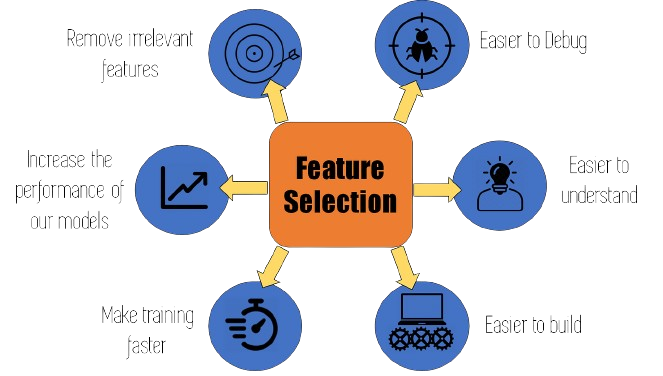
\includegraphics[width=\textwidth]{imagenes/chapter1/feature_selection_pros-removebg-preview.png}
      \end{center}
      \caption{Beneficios de la selección de características}
    \end{figure}
  \end{columns}
  \vspace{-.2cm}
\end{frame}

\note{

}

\subsection{Motivación}
\begin{frame}
  \frametitle{Motivación}
  \begin{enumerate}
    \item \textbf{La selección de características} es un procesamiento esencial en el aprendizaje automático
    \item Muchos algoritmos y métodos abordar el problema. Nos centramos en
          metaheurísticas
    \item No hay gran número de comparaciones entre versiones binarias y continuas
    \item Poca rigurosidad en comparaciones existentes
  \end{enumerate}
  \vspace{-.2cm}
\end{frame}

\begin{frame}
  \frametitle{Motivación}
  \begin{enumerate}
    \item Identificamos propuestas novedosas (problemas continuos)
    \item Implementamos versiones binarias de las anteriores
    \item Comparación rigurosas entre algoritmos:
          \begin{itemize}
            \item Distintas métricas
            \item Test estadísticos
          \end{itemize}
  \end{enumerate}
  \vspace{-.2cm}
\end{frame}

\subsection{Búsquedas Scopus}
\begin{frame}
  \frametitle{Tendencia Scopus}
  \begin{columns}
    \column{0.5\textwidth}
    \begin{figure}
      \begin{center}
        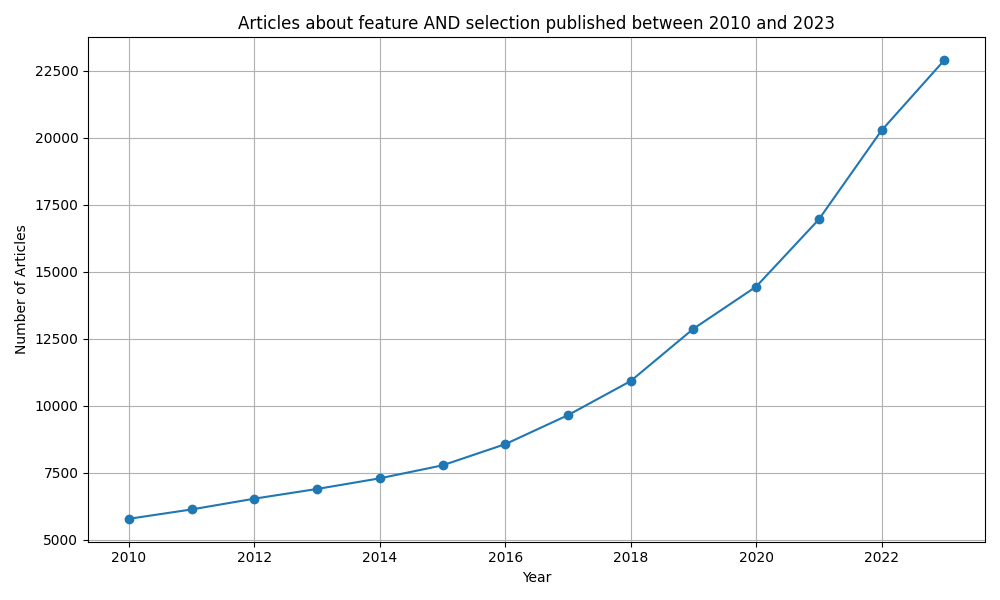
\includegraphics[width=\textwidth]{imagenes/chapter3/scopus_chart.png}
      \end{center}
      \caption{Tendencia en artículos publicados de \textbf{feature selection} en Scopus. Se incrementa exponencialmente con el tiempo.}
    \end{figure}

    \column{0.5\textwidth}
    \begin{figure}
      \begin{center}
        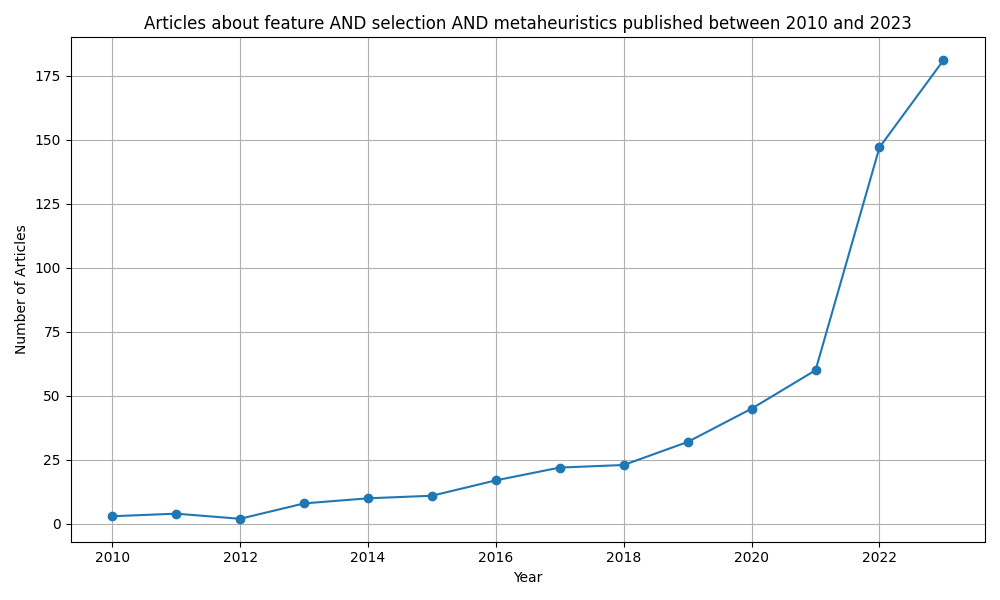
\includegraphics[width=\textwidth]{imagenes/chapter3/scopus_chart2.png}
      \end{center}
      \caption{Tendencia en artículos publicados sobre \textbf{feature selection} usando \textbf{metaheurísticas} en Scopus.}
    \end{figure}
  \end{columns}
\end{frame}

\note{

}

\note{

}

\subsection{Objetivos}
\begin{frame}
  \frametitle{Objetivos}
  \begin{columns}
    \column{0.6\textwidth}
    \begin{enumerate}
      \item Evaluar el desempeño de las metaheurísticas
      \item Investigar versiones continuas y binarias
      \item Fortalezas y debilidades de las metaheurísticas
      \item Recomendaciones prácticas según el contexto
      \item Evaluación de resultados finales y realizar comparaciones
      \item Resolver una serie de preguntas de investigación. ¿Binarios vs. continuos?
    \end{enumerate}
    \column{0.6\textwidth}
    \begin{figure}
      \begin{center}
        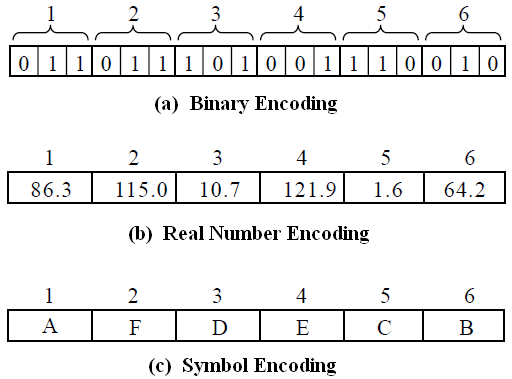
\includegraphics[width=0.7\textwidth]{imagenes/chapter1/real_vs_bin.png}
      \end{center}
      \caption{Codificaciones binarias y continuas\footnotemark[1]}
    \end{figure}
  \end{columns}
  \footnotetext[1]{\cite{binary_real}}
\end{frame}

\note{

}

\subsection{Metaheurísticas}
\begin{frame}
  \frametitle{¿Qué son las metaheurísticas?}
  \begin{columns}
    \column{0.6\textwidth}
    \begin{enumerate}
      \item Las metaheurísticas son algoritmos de \textbf{optimización}
      \item Suelen estar bioinspiradas
      \item Son algoritmos generales que no dependen de un dominio en un problema específico
      \item Consiguen soluciones muy buenas en tiempos razonables
    \end{enumerate}
    \column{0.4\textwidth}
    \begin{figure}
      \begin{center}
        \animategraphics[loop, autoplay, width=0.8\textwidth]{10}{imagenes/chapter1/ParticleSwarmArrowsAnimation-}{0}{99}
      \end{center}
      \caption{Algoritmo PSO en busca del \textbf{mínimo} de una función\footnotemark[2]}
    \end{figure}
  \end{columns}
  \footnotetext[2]{\cite{wiki:PSO}}
\end{frame}

\note{

}

\begin{frame}
  \frametitle{Tipos de mateheurísticas}
  \begin{columns}
    \column{0.4\textwidth}
    \begin{figure}
      \begin{center}
        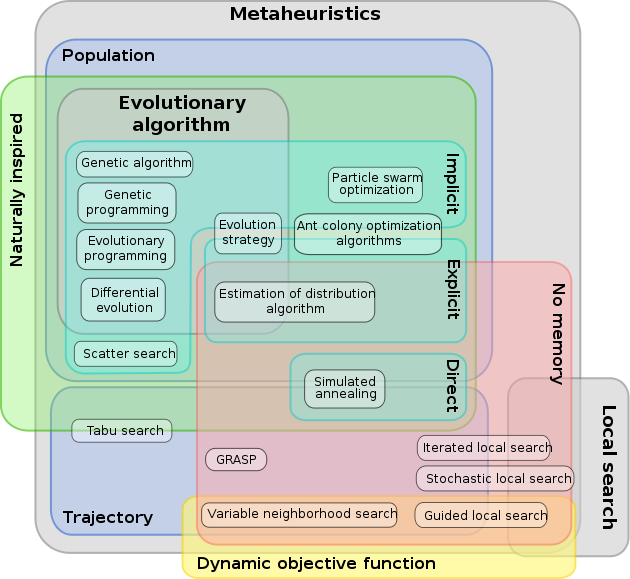
\includegraphics[width=1\textwidth]{imagenes/chapter1/mh_euler_graph.png}
      \end{center}
      \caption{Tipos de metaheurísticas}
    \end{figure}
    \column{0.6\textwidth}
    \begin{enumerate}
      \item Las metaheurísticas seleccionadas en este proyecto son todas del tipo \textbf{poblacional} y evolutivas
    \end{enumerate}
  \end{columns}
\end{frame}

\note{

}


\note{

}
\section{Planificación}
\subsection{Presupuesto y planificación}

\begin{frame}
    \frametitle{Tareas}
    \begin{table}[htp]
        \centering
        \begin{tabular}{c|c|c}
            Tarea                         & Duración Prevista (h) & Duración Final (h) \\ \hline
            Investigación inicial         & 20                    & 20                 \\
            Diseño del software           & 10                    & 10                 \\
            Investigación metaheurísticas & 60                    & 60                 \\
            Implementación del software   & 70                    & 90                 \\
            Pruebas y refactorizado       & 15                    & 25                 \\
            Análisis de resultados        & 40                    & 20                 \\
            Documentación                 & 90                    & 120                \\ \hline
        \end{tabular}
        \caption{Tabla de duración de cada tarea}
        \label{tab:task_duration}
    \end{table}
\end{frame}

\begin{frame}
    \frametitle{Diagrama de Gantt}
    \begin{figure}
        \centering
        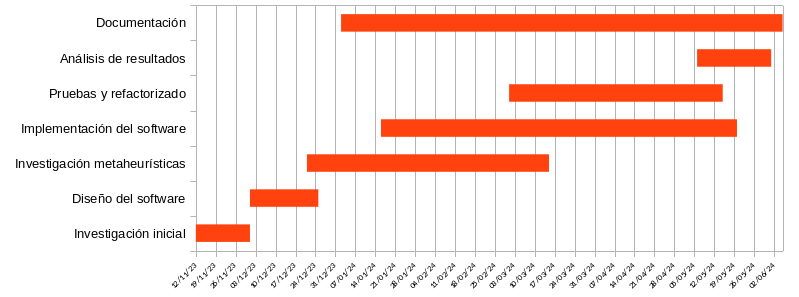
\includegraphics[width=0.8\textwidth]{imagenes/chapter2/gantt-fin.png}
        \caption{Diagrama de Gantt}
    \end{figure}
\end{frame}

\begin{frame}
    \frametitle{Presupuesto}
    \begin{columns}
        \column{1\textwidth}
        \begin{itemize}
            \item \textbf{Sueldo}: $25$€/hora, $340$ horas, total $8.500$€
            \item \textbf{Portátil}: HP Pavilion, $1000$€, usado $8$ meses, costo $133.3$€
            \item \textbf{Servidor}: Uso del servidor \textbf{Hércules}, costo real cero. Estimación en \textit{Google Cloud}
        \end{itemize}
    \end{columns}
\end{frame}

\note{

}

\begin{frame}
    \frametitle{Presupuesto}
    \begin{columns}
        \column{1\textwidth}
        \begin{table}[htp]
            \centering
            \begin{tabular}{|l|r|}
                \hline
                \textbf{Item}                    & \textbf{Costo (€)} \\ \hline
                Salario                          & 8500               \\
                Ordenador portátil               & 133.3              \\
                Servidor CPU - GC Compute Engine & 75.84              \\
                \textbf{Total}                   & \textbf{8709.14}   \\ \hline
            \end{tabular}
            \caption{Costo estimado del proyecto}
        \end{table}
    \end{columns}
\end{frame}
\section{Revisión de la literatura}

\begin{frame}
  \frametitle{Ventajas actuales de las Metaheurísticas}
  \begin{columns}
    \column{0.5\textwidth}
    \begin{figure}
      \begin{center}
        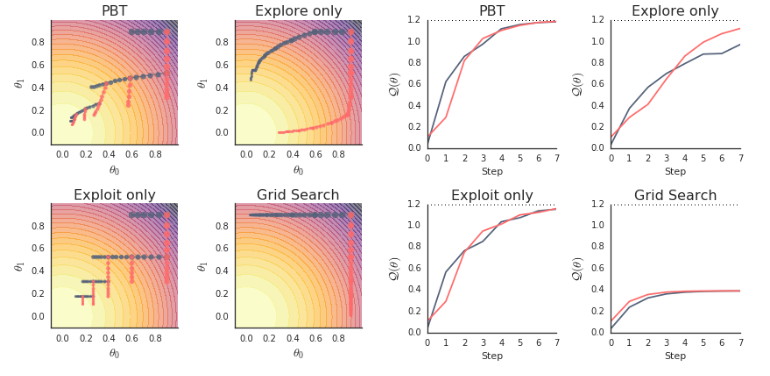
\includegraphics[width=\textwidth]{imagenes/chapter3/pbt.png}
      \end{center}
      \caption{Uso de algoritmo poblacional \textbf{PBT} en búsqueda de hiperparámetros \footnotemark[3]}
    \end{figure}
    \column{0.5\textwidth}
    \begin{itemize}
      \item \textbf{Implementación práctica}: Utilizadas en aplicaciones reales, como la planificación de rutas, diseño de redes y gestión de recursos
      \item \textbf{Integración con AI}: Combinadas con técnicas de inteligencia artificial para mejorar el rendimiento
      \item \textbf{Adaptabilidad}: Ajustables a problemas específicos mediante parametrización de los cuales no es posible obtener funciones de pérdida diferenciables
    \end{itemize}
  \end{columns}
  \footnotetext[3]{\cite{Mafarja201825}}
\end{frame}

\note{

}

\subsection{Algoritmos}
\begin{frame}
  \frametitle{Algoritmos seleccionados}
  \begin{enumerate}
    \item Se escogen para el proyecto una serie de algoritmos basándose en la investigación de aquellos más novedosos, con mejor rendimiento y más citados. Estos son los que se denominarán \textbf{modernos}
    \item Además de los algoritmos más novedosos, se incluyen una serie de algoritmos clásicos, cuyo robustez a lo largo de los años tras multitud de aplicaciones en problemas es notable. Esta categoría, es la de los algoritmos \textbf{clásicos}
  \end{enumerate}
\end{frame}

\begin{frame}
  \frametitle{Grey Wolf Optimizer}
  \begin{columns}
    \column{0.5\textwidth}
    \begin{enumerate}
      \item Inspirado en el comportamiento social y la técnica de caza de los lobos grises
      \item Modela una \textbf{jerarquía social} para guiar la búsqueda de soluciones óptimas, donde los lobos alfa, beta y delta lideran el proceso de exploración y explotación
    \end{enumerate}
    \column{0.5\textwidth}
    \begin{figure}
      \begin{center}
        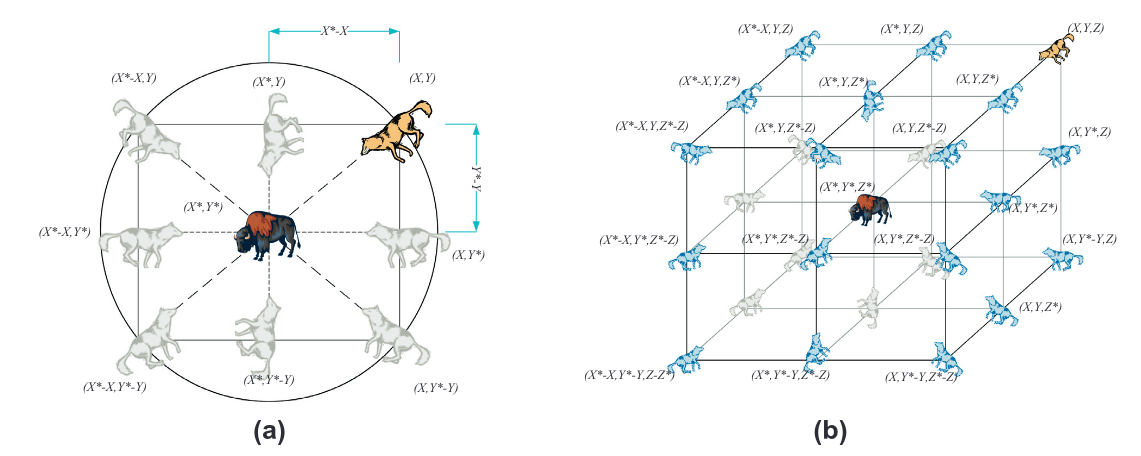
\includegraphics[width=\textwidth]{imagenes/chapter3/grey-wolf-hunt.png}
      \end{center}
      \caption{Caza de los lobos grises \footnotemark[4]}
    \end{figure}
  \end{columns}
  \footnotetext[4]{\cite{mirjalili_grey_2014}}
\end{frame}

\begin{frame}
  \frametitle{Grasshopper Optimization Algorithm}
  \begin{columns}
    \column{0.5\textwidth}
    \begin{figure}
      \begin{center}
        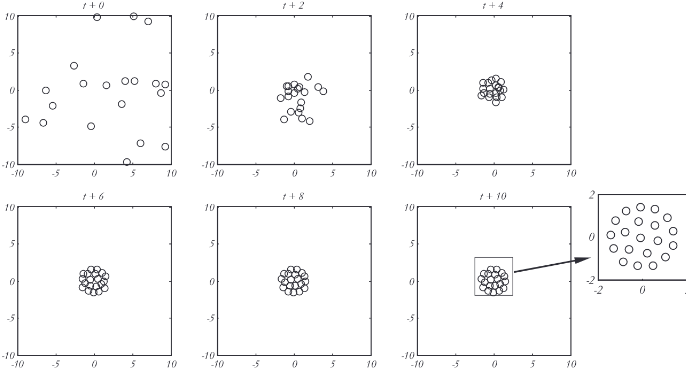
\includegraphics[width=\textwidth]{imagenes/chapter3/goa-position-convergence.png}
      \end{center}
      \caption{Convergencia de los saltamontes \footnotemark[5]}
    \end{figure}
    \column{0.5\textwidth}
    \begin{enumerate}
      \item Simula el movimiento y la interacción de los saltamontes en sus distintas etapas de vida
    \end{enumerate}
  \end{columns}
  \footnotetext[5]{\cite{saremi_grasshopper_2017}}
\end{frame}

\begin{frame}
  \frametitle{Firefly Algorithm}
  \begin{columns}
    \column{0.5\textwidth}
    \begin{enumerate}
      \item Inspirado en el comportamiento de \textbf{parpadeo} y \textbf{atracción} de las luciérnagas
      \item Utiliza la intensidad de la luz como guía para la atracción entre luciérnagas, donde las luciérnagas menos brillantes se mueven hacia las más brillantes
    \end{enumerate}
    \column{0.5\textwidth}
    \begin{figure}
      \begin{center}
        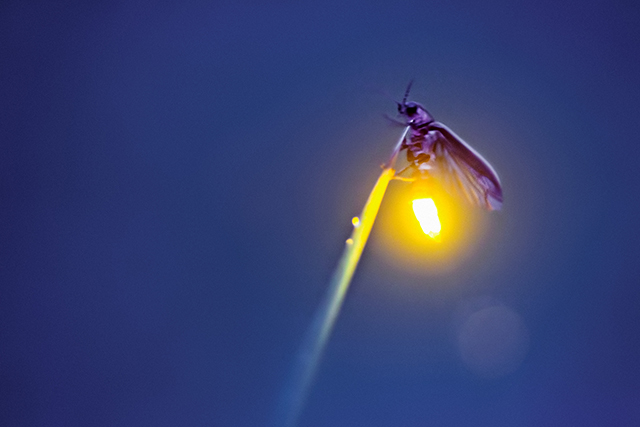
\includegraphics[width=\textwidth]{imagenes/chapter3/firefly.jpg}
      \end{center}
      \caption{Imagen de una libélula con su característico brillo}
    \end{figure}
  \end{columns}
\end{frame}

\begin{frame}
  \frametitle{Cuckoo Search}
  \begin{columns}
    \column{0.5\textwidth}
    \begin{figure}
      \begin{center}
        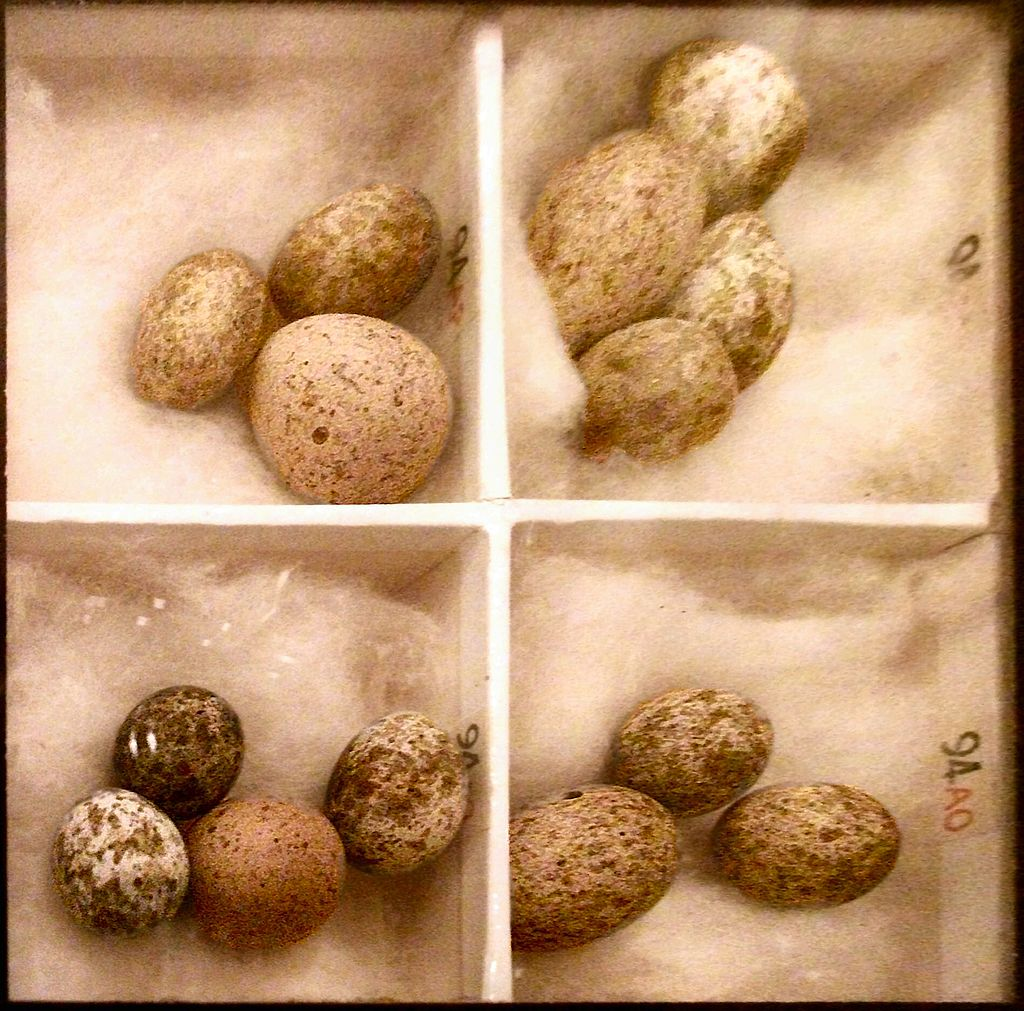
\includegraphics[width=0.6\textwidth]{imagenes/chapter3/cucko_eggs.jpg}
      \end{center}
      \caption{Cuatro nidos de huevos de pájaro. En cada uno de ellos un huevo visiblemente más grande del pájaro Cuco \footnotemark[6]}
    \end{figure}
    \column{0.5\textwidth}
    \begin{enumerate}
      \item Inspirado en el comportamiento de anidación de los cucos y el \textbf{parasitismo} de puesta
      \item Caracterizado por usar métodos de búsqueda aleatoria y el método \textbf{Levy flight} para la exploración del espacio de soluciones
    \end{enumerate}
  \end{columns}
  \footnotetext[6]{\cite{chiswickchap_cuckooeggs_2024}}
\end{frame}

\begin{frame}
  \frametitle{Genetic Algorithm}
  \begin{columns}
    \column{0.5\textwidth}
    \begin{enumerate}
      \item Algoritmo basado en la recombinación de cromosomas, que toma inspiración de la \textbf{evolución} biológica y genética
      \item Hace uso de operadores tales como la \textbf{mutación} o el \textbf{cruce}
    \end{enumerate}
    \column{0.5\textwidth}
    \begin{figure}
      \begin{center}
        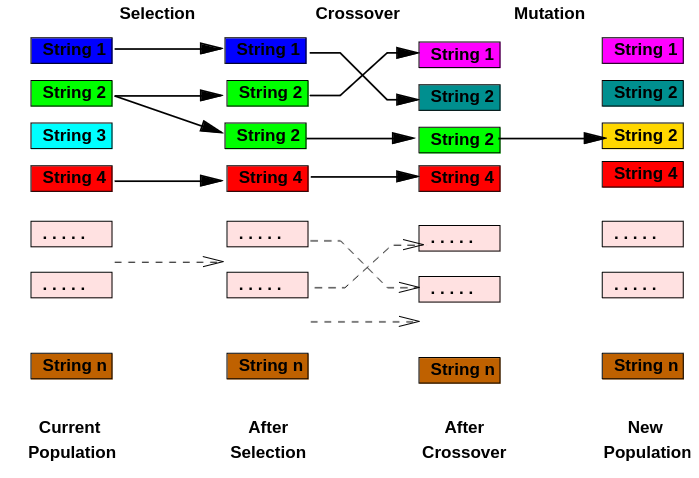
\includegraphics[width=\textwidth]{imagenes/chapter3/ga-working-principle.png}
      \end{center}
      \caption{Principio básico del algoritmo GA \footnotemark[7]}
    \end{figure}
  \end{columns}
  \footnotetext[7]{\cite{mathew2012genetic}}
\end{frame}

\begin{frame}
  \frametitle{Whale Optimization Algorithm}
  \begin{columns}
    \column{0.5\textwidth}
    \begin{figure}
      \begin{center}
        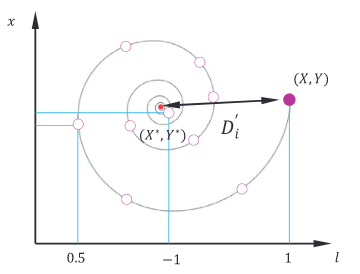
\includegraphics[width=0.7\textwidth]{imagenes/chapter3/spiral-update-position-wao.png}
      \end{center}
      \caption{Espiral para simular el mecanismo de ataque de la red de burbujas de las ballenas jorobadas \footnotemark[8]}
    \end{figure}
    \column{0.5\textwidth}
    \begin{enumerate}
      \item Inspirado en el comportamiento de las ballenas jorobadas
      \item Usa principalmente dos variantes de operadores de caza:
            \begin{itemize}
              \item \textbf{Espiral de búsqueda}
              \item \textbf{Técnica de burbujeo de red}
            \end{itemize}
    \end{enumerate}
  \end{columns}
  \footnotetext[8]{\cite{mirjalili_whale_2016}}
\end{frame}

\begin{frame}
  \frametitle{Artificial Bee Colony Optimization}
  \begin{columns}
    \column{0.5\textwidth}
    \begin{enumerate}
      \item Simula la \textbf{búsqueda de alimentos} de las abejas empleadas, las abejas observadoras y las abejas exploradoras para encontrar soluciones óptimas
    \end{enumerate}
    \column{0.5\textwidth}
    \begin{figure}
      \begin{center}
        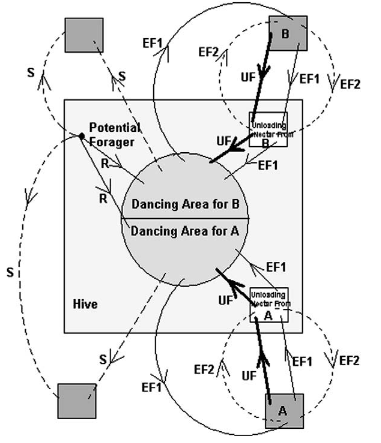
\includegraphics[width=0.5\textwidth]{imagenes/chapter3/abco.png}
      \end{center}
      \caption{Diagrama de funcionamiento del ABCO \footnotemark[9]}
    \end{figure}
  \end{columns}
  \footnotetext[9]{\cite{Karaboga2009108}}
\end{frame}


\begin{frame}
  \frametitle{Dragonfly Algorithm}
  \begin{columns}
    \column{0.5\textwidth}
    \begin{figure}
      \begin{center}
        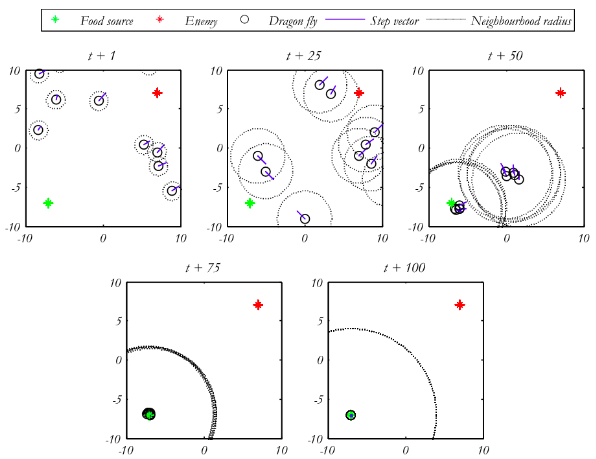
\includegraphics[width=0.7\textwidth]{imagenes/chapter3/da-operators.png}
      \end{center}
      \caption{Operadores del algoritmo DA \footnotemark[10]}
    \end{figure}
    \column{0.5\textwidth}
    \begin{enumerate}
      \item Basado en el comportamiento de enjambre y formación de las libélulas, usando operadores que controlan características como la \textbf{cohesión} de grupo o \textbf{distanciamiento} del enemigo, entre otros
      \item Simula las interacciones sociales y el movimiento de las libélulas para equilibrar la exploración y explotación del espacio de soluciones
    \end{enumerate}
  \end{columns}
  \footnotetext[10]{\cite{Meraihi2020}}
\end{frame}

\begin{frame}
  \frametitle{Ant Colony Optimization}
  \begin{columns}
    \column{0.5\textwidth}
    \begin{enumerate}
      \item Simula las colonias de hormigas. Para ello usa el rastro de \textbf{feromonas} para guiar la búsqueda de soluciones óptimas, donde las hormigas depositan y siguen feromonas en los caminos más prometedores
    \end{enumerate}
    \column{0.5\textwidth}
    \begin{figure}
      \begin{center}
        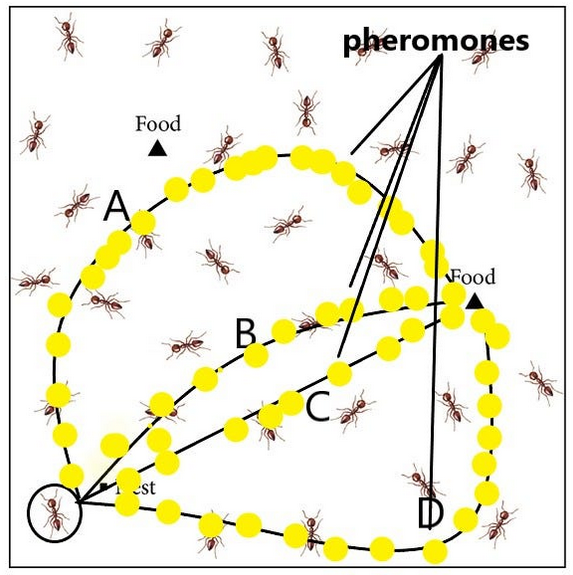
\includegraphics[width=0.5\textwidth]{imagenes/chapter3/aco.png}
      \end{center}
      \caption{Caminos de un grafo marcados por la feromona, operador esencial de ACO}
    \end{figure}
  \end{columns}
\end{frame}

\begin{frame}
  \frametitle{Particle Swarm Optimization}
  \begin{columns}
    \column{0.5\textwidth}
    \begin{figure}
      \begin{center}
        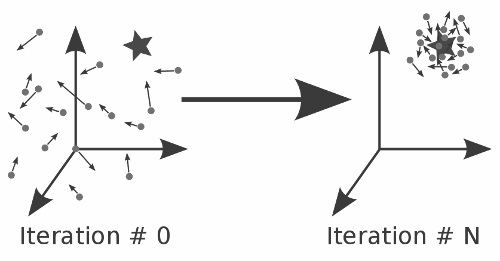
\includegraphics[width=0.7\textwidth]{imagenes/chapter3/pso.png}
      \end{center}
      \caption{Partículas en el espacio (con una velocidad y dirección) convergiendo en la iteración $N$}
    \end{figure}
    \column{0.5\textwidth}
    \begin{enumerate}
      \item Inspirado en el comportamiento social de los enjambres de aves y peces
      \item Simula la búsqueda colectiva de soluciones, donde cada partícula ajusta su posición basada en su \textbf{experiencia} personal y la de sus \textbf{vecinos}
    \end{enumerate}
  \end{columns}
\end{frame}

\begin{frame}
  \frametitle{Bat Algorithm}
  \begin{columns}
    \column{0.5\textwidth}
    \begin{enumerate}
      \item Basado en el comportamiento de \textbf{ecolocalización} de los murciélagos
      \item Utiliza la técnica de emisión de pulsos y el ajuste de frecuencia para explorar y explotar el espacio de soluciones
    \end{enumerate}
    \column{0.5\textwidth}
    \begin{figure}
      \begin{center}
        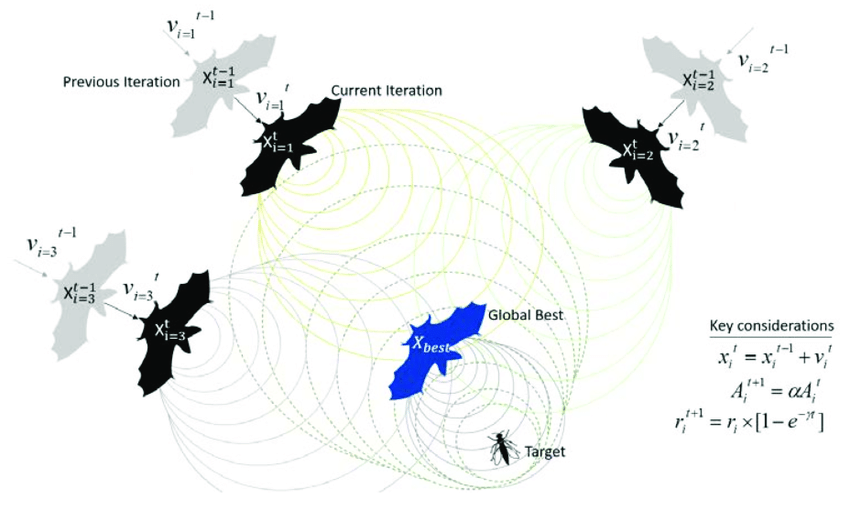
\includegraphics[width=0.9\textwidth]{imagenes/chapter3/ba.png}
      \end{center}
      \caption{Funcionamiento del algoritmo BA}
    \end{figure}
  \end{columns}
\end{frame}

\begin{frame}
  \frametitle{Differential Evolution}
  \begin{columns}
    \column{0.5\textwidth}
    \begin{figure}
      \begin{center}
        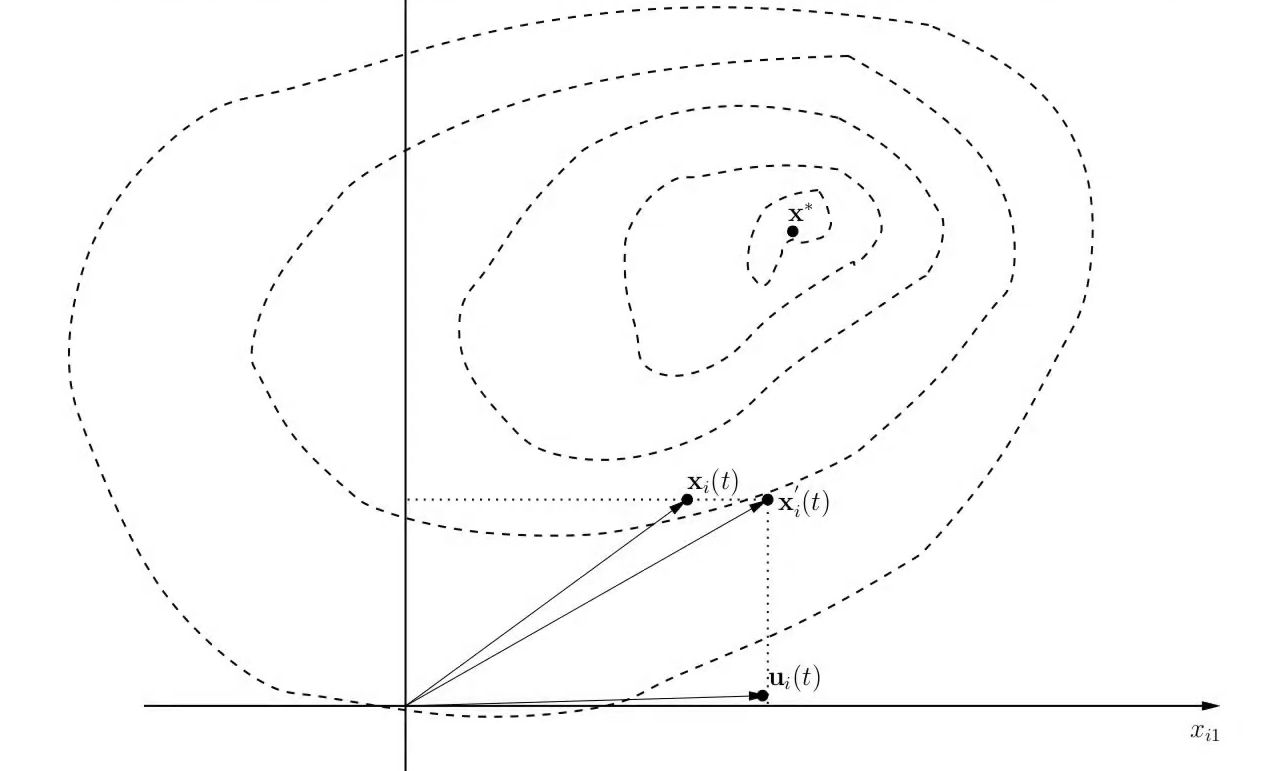
\includegraphics[width=1\textwidth]{imagenes/chapter3/de-crossover.png}
      \end{center}
      \caption{Operador de \textit{crossover} o cruce de DE \footnotemark[11]}
    \end{figure}
    \column{0.5\textwidth}
    \begin{enumerate}
      \item Utiliza la combinación y mutación de vectores solución para buscar la mejor solución, enfocándose en la \textbf{diferencia} entre las soluciones actuales para generar nuevas
    \end{enumerate}
  \end{columns}
  \footnotetext[11]{\cite{10.5555/1557464}}
\end{frame}
\section{Diseño Experimental}
\subsection{Conjuntos de datos}
\begin{frame}
  \frametitle{Conjuntos de datos}
  \begin{columns}
    \column{0.5\textwidth}
    \begin{enumerate}
      \item Se escogen conjuntos de datos por:
            \begin{itemize}
              \item \textbf{Variedad de áreas}
              \item \textbf{Diversidad de problemas}
              \item \textbf{Número de características}
              \item \textbf{Relevancia práctica}
            \end{itemize}
    \end{enumerate}
    \column{0.5\textwidth}
    \begin{table}[htp]
      \centering
      \tiny
      \setlength{\tabcolsep}{4pt}
      \begin{tabular}{ l r r r l }
        \hline
        \textbf{Dataset} & \textbf{Inst.} & \textbf{Car.} & \textbf{Cls.} & \textbf{Área} \\ \hline
        sonar            & 207            & 60            & 2             & Biología      \\
        spambase-460     & 459            & 54            & 2             & Informática   \\
        spectf-heart     & 348            & 44            & 2             & Medicina      \\
        waveform5000     & 5000           & 40            & 3             & Física        \\
        ionosphere       & 350            & 34            & 2             & Meteorología  \\
        dermatology      & 366            & 34            & 6             & Medicina      \\
        wdbc             & 568            & 29            & 2             & Medicina      \\
        parkinsons       & 200            & 22            & 2             & Medicina      \\
        zoo              & 101            & 18            & 7             & Biología      \\
        wine             & 182            & 13            & 3             & Alimentación  \\
        breast-cancer    & 286            & 9             & 2             & Medicina      \\
        diabetes         & 768            & 8             & 2             & Medicina      \\
        yeast            & 1483           & 8             & 10            & Biología      \\
        ecoli            & 336            & 7             & 8             & Biología      \\
        iris             & 149            & 4             & 3             & Biología      \\ \hline
      \end{tabular}
      \caption{Información de conjuntos de datos por número de características}
      \label{tab:datasets_info}
    \end{table}
  \end{columns}
\end{frame}

\begin{frame}
  \frametitle{Diseño Experimental}
  \begin{enumerate}
    \item La función \textit{fitness} se construye con:
          \begin{itemize}
            \item \textbf{Accuracy} al $90\%$.
            \item \textbf{Reducción} al $10\%$.
          \end{itemize}
    \item Se define como: \begin{equation}
            fitness = acc\cdot\alpha + red\cdot(1-\alpha)
            \label{eq:fitness}
          \end{equation}
          Donde $\alpha$ es la ponderación dada a la precisión o \textit{accuracy}.
  \end{enumerate}
\end{frame}
\section{Resultados y Análisis}

\subsection{Continuos}

\begin{frame}
    \frametitle{Ranking en continuos para fitness}
    \begin{columns}
        \column{0.5\textwidth}
        \begin{figure}
            \begin{center}
                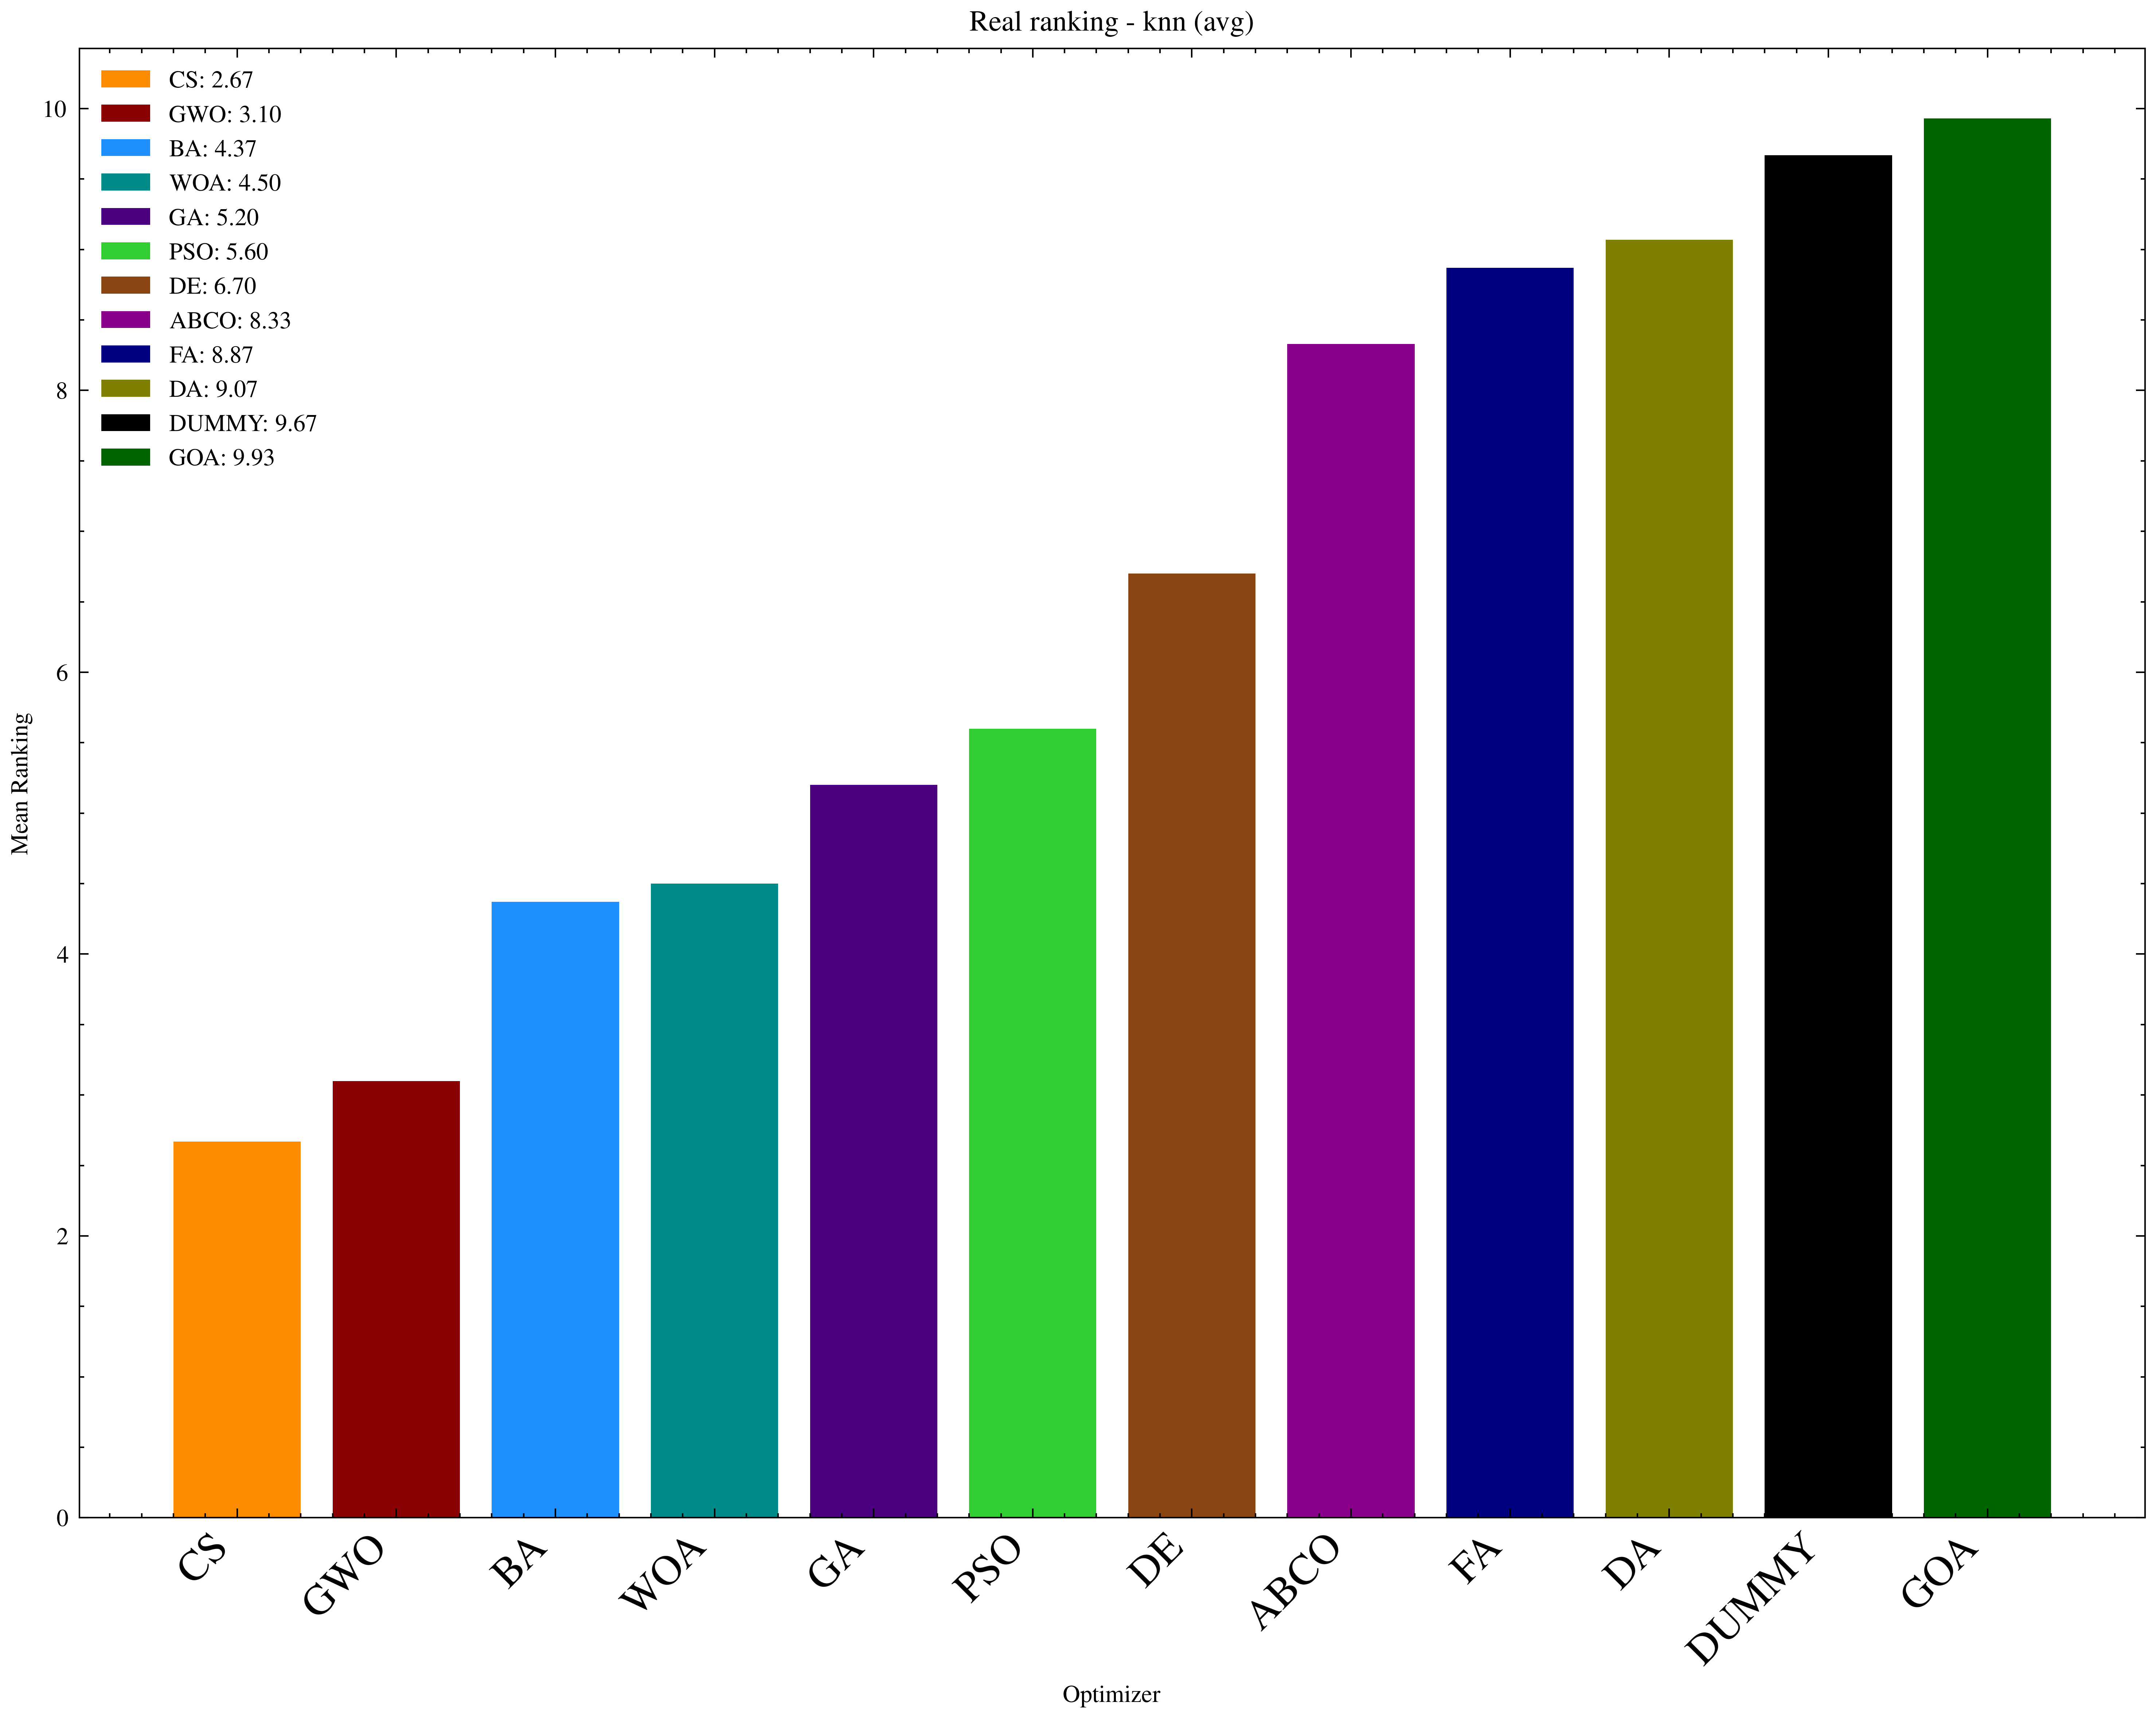
\includegraphics[width=0.8\textwidth]{imagenes/chapter5/rankings_knn_avg_real.png}
            \end{center}
            \caption{Ranking de los algoritmos en versión continua para kNN}
        \end{figure}
        \column{0.5\textwidth}
        \begin{figure}
            \begin{center}
                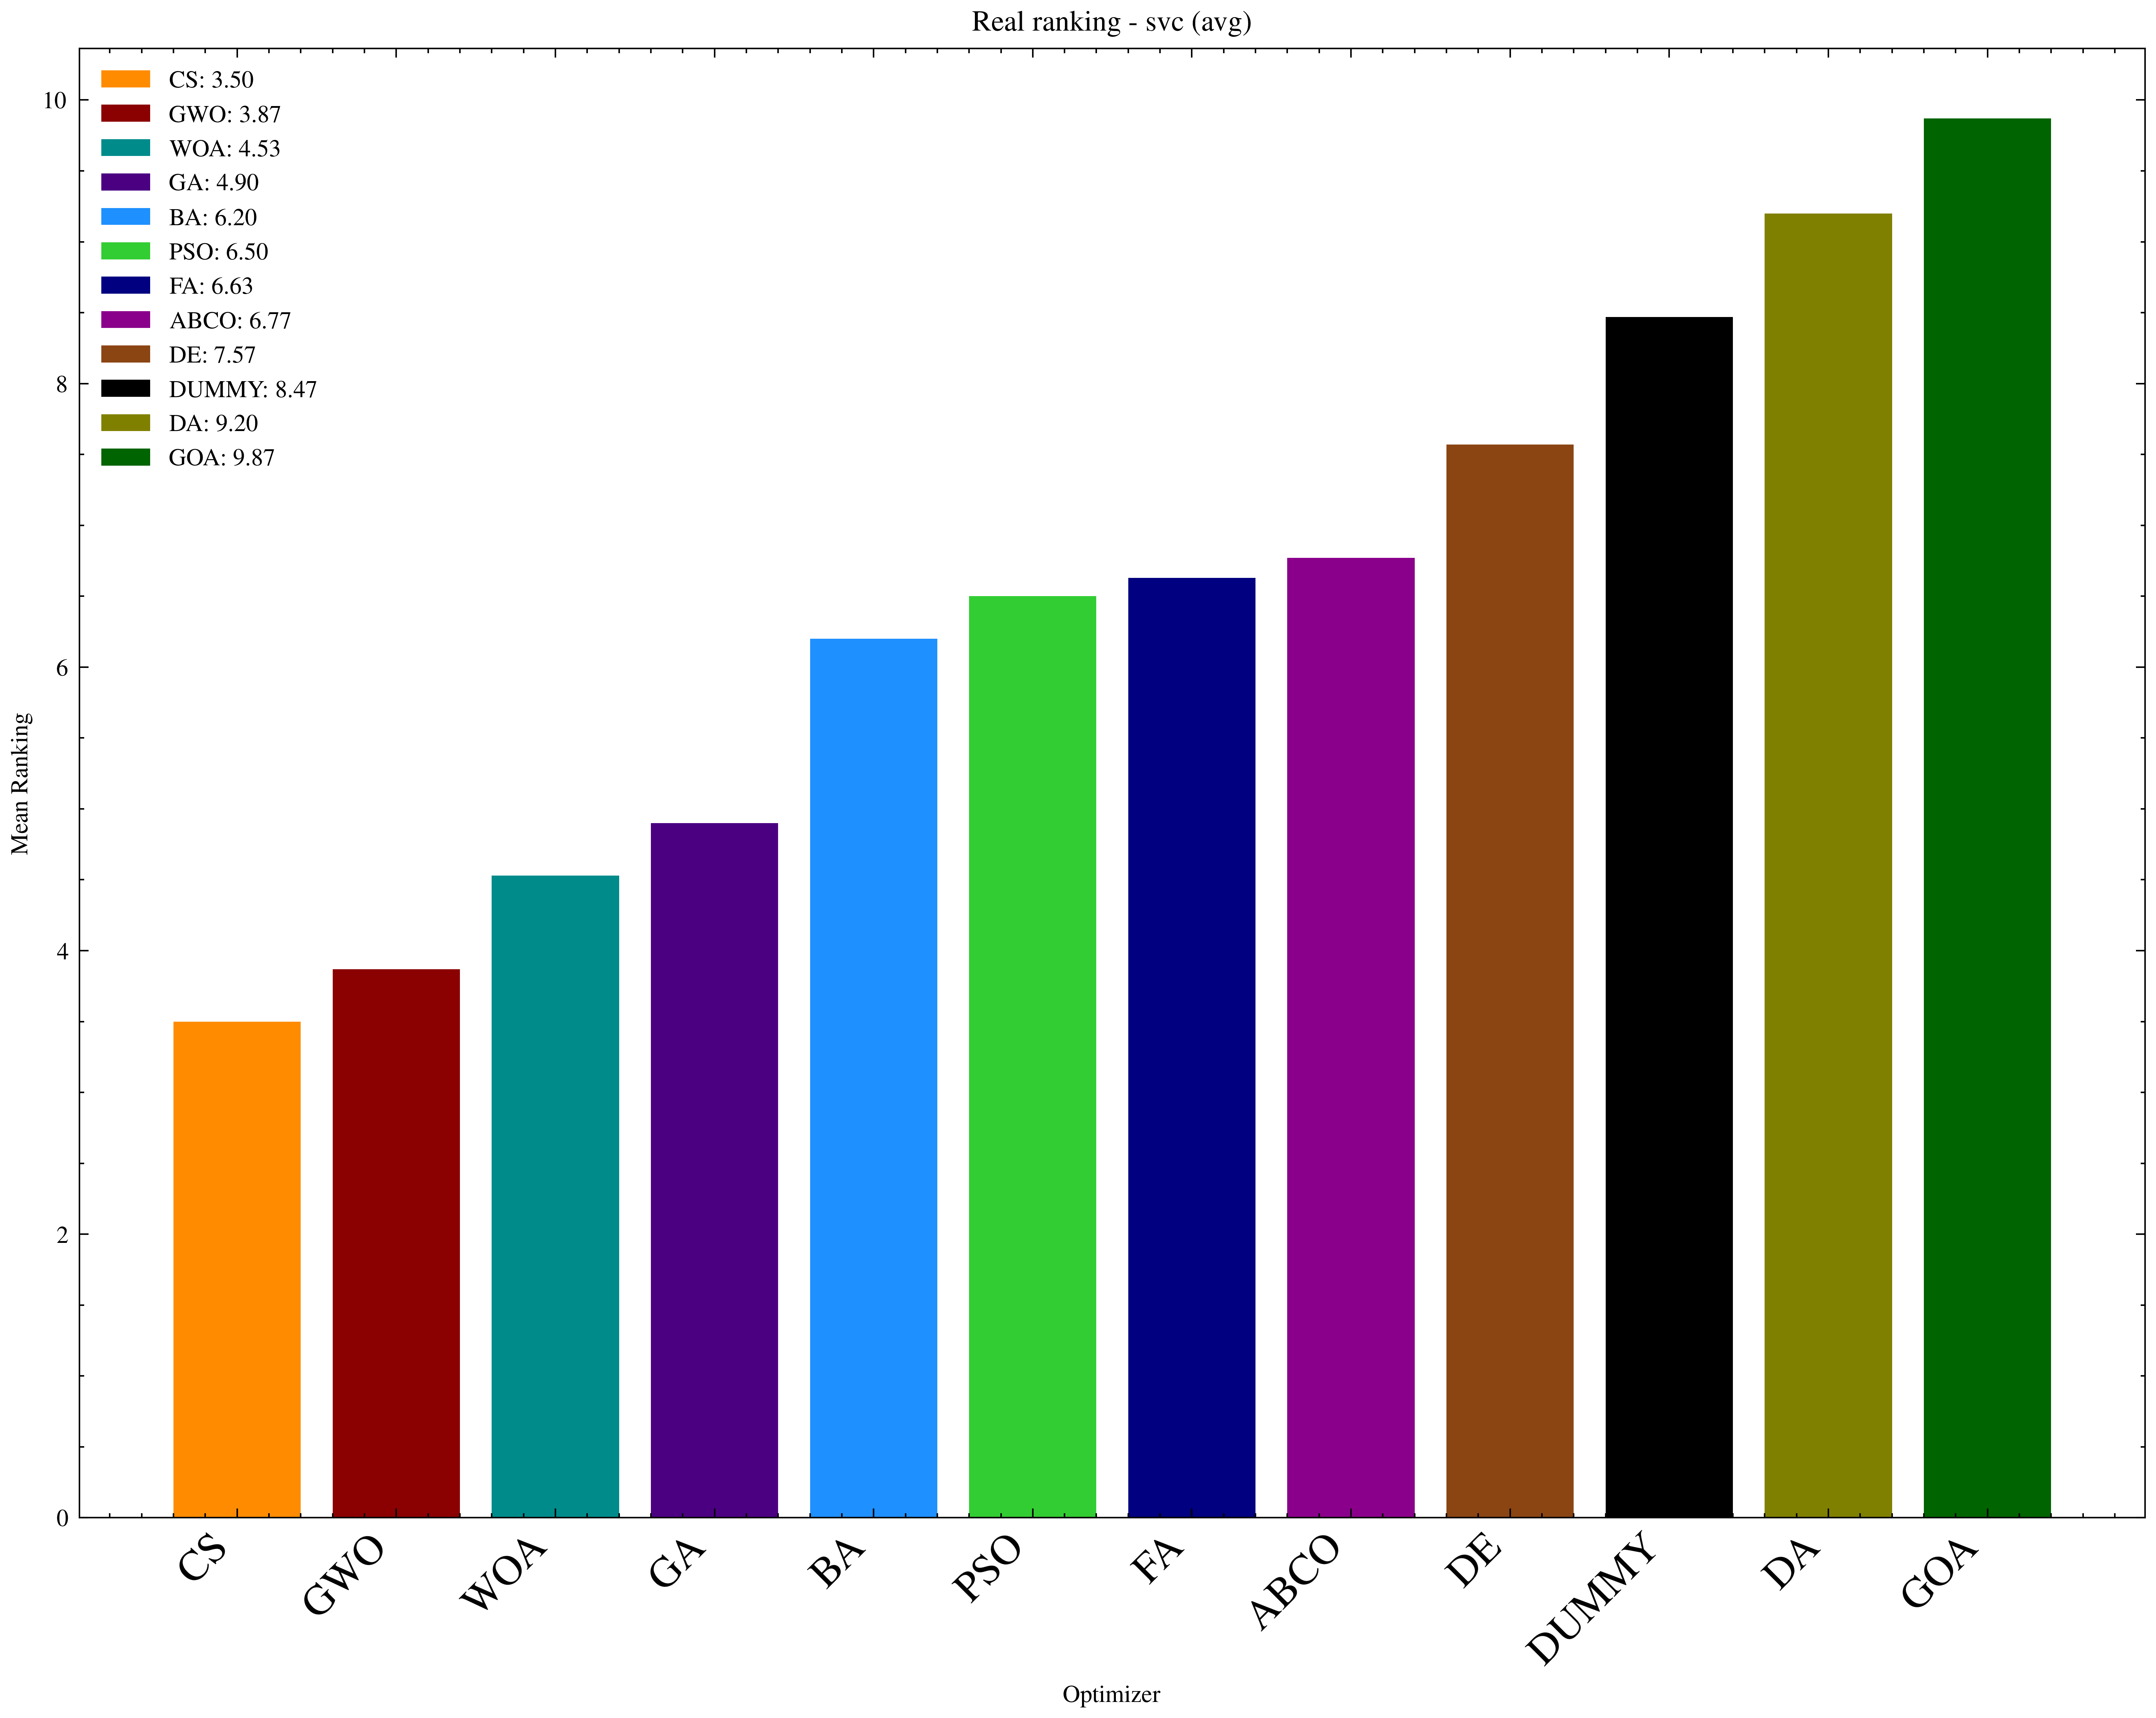
\includegraphics[width=0.8\textwidth]{imagenes/chapter5/rankings_svc_avg_real.png}
            \end{center}
            \caption{Ranking de los algoritmos en versión continua para SVC}
        \end{figure}
    \end{columns}
\end{frame}

\begin{frame}
    \frametitle{Resultados en continuos}
    \begin{enumerate}
        \item Los mejores algoritmos en \textit{fitness} son \textbf{CS} y \textbf{GWO}. Los peores algoritmos son \textbf{GOA} y \textbf{DA}.
        \item Los mejores reduciendo características vuelven a ser \textbf{CS} y \textbf{GWO}. Además con mucha diferencia.
        \item El algoritmo más rápido es \textbf{FA}, mientras que el más lento es \textbf{ABCO}.
    \end{enumerate}
\end{frame}


\begin{frame}
    \frametitle{Convergencia en continuo}
    \begin{columns}
        \column{0.5\textwidth}
        \begin{figure}[htp]
            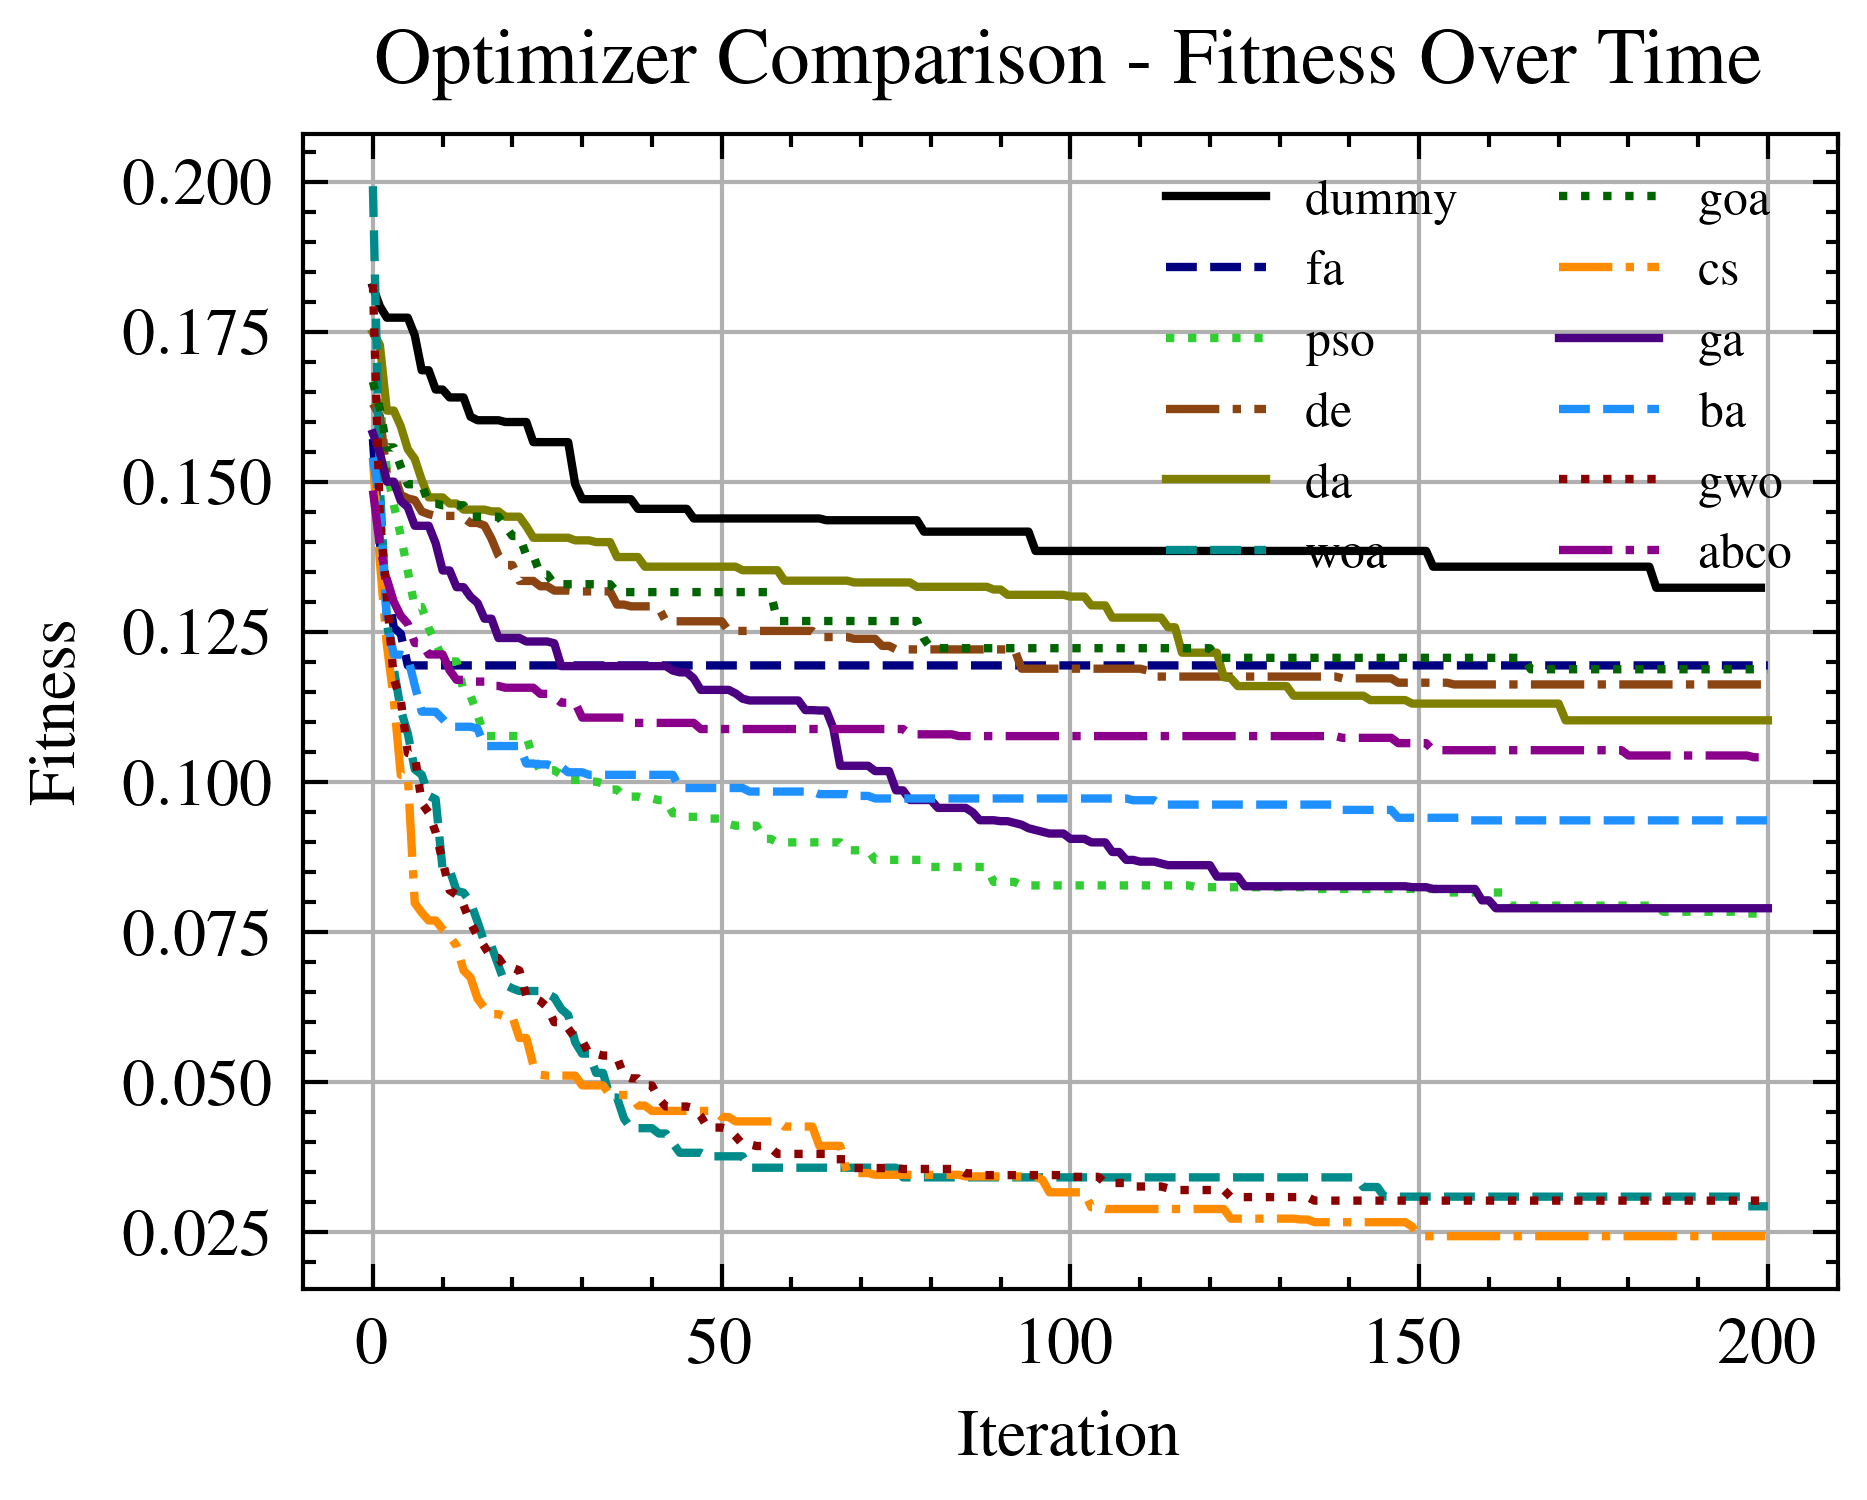
\includegraphics[width=0.8\textwidth]{imagenes/chapter5/optimizers_fitness_knn_io.png}
            \caption{Convergencia de todas las metaheurísticas en ionosphere - knn - real}
        \end{figure}
        \column{0.5\textwidth}
        \begin{figure}[htp]
            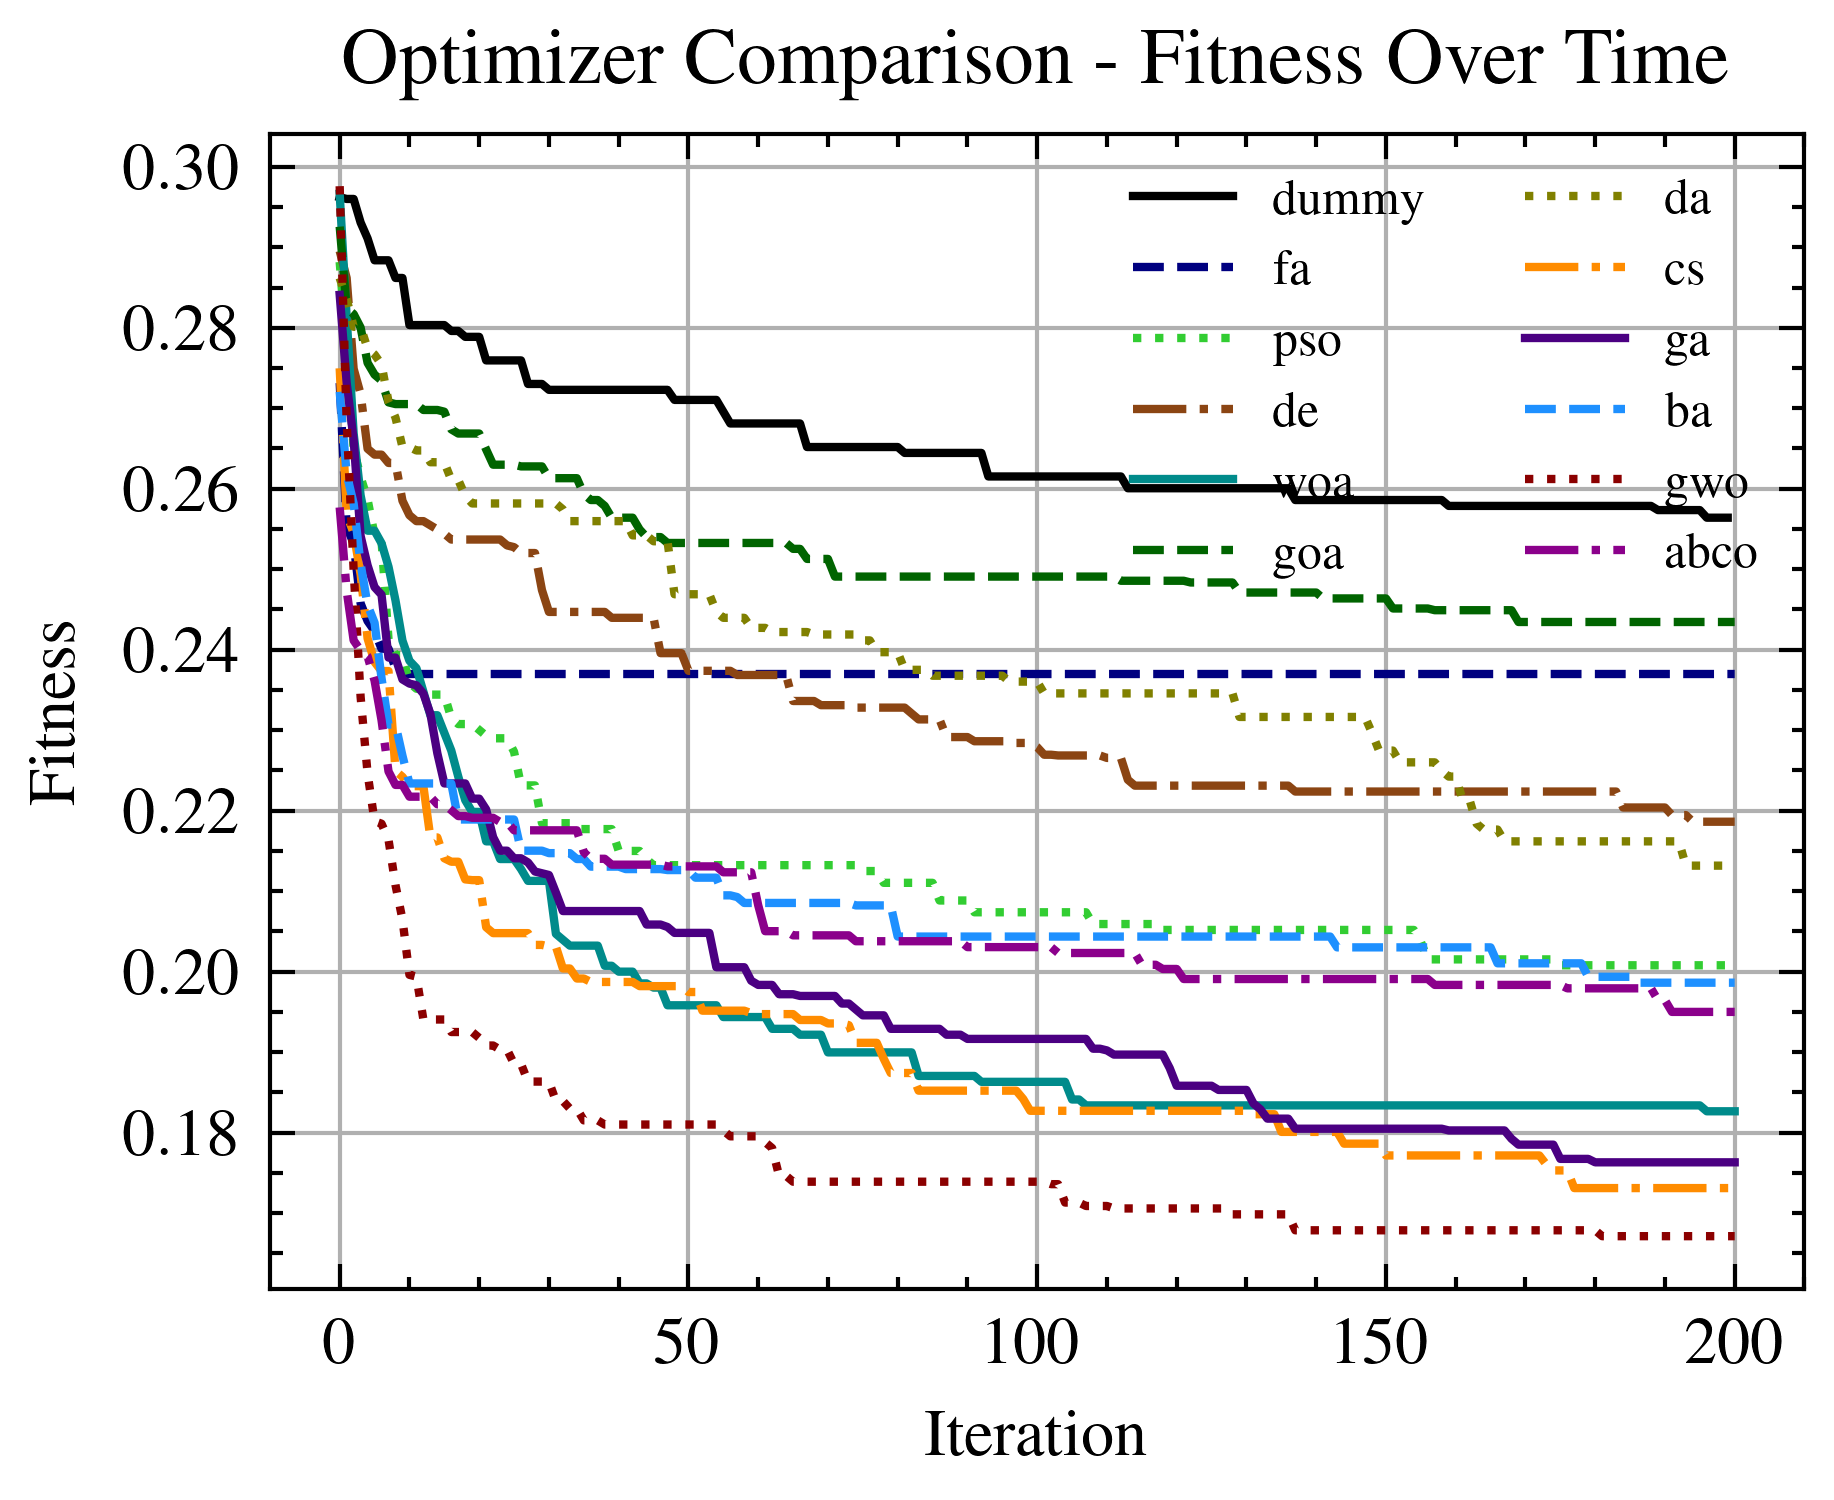
\includegraphics[width=0.8\textwidth]{imagenes/chapter5/optimizers_fitness_knn_dia.png}
            \caption{Convergencia de todas las metaheurísticas en diabetes - knn - real}
        \end{figure}
    \end{columns}
\end{frame}


\subsection{Binarios}
\begin{frame}
    \frametitle{Ranking en binario para fitness}
    \begin{columns}
        \column{0.5\textwidth}
        \begin{figure}
            \begin{center}
                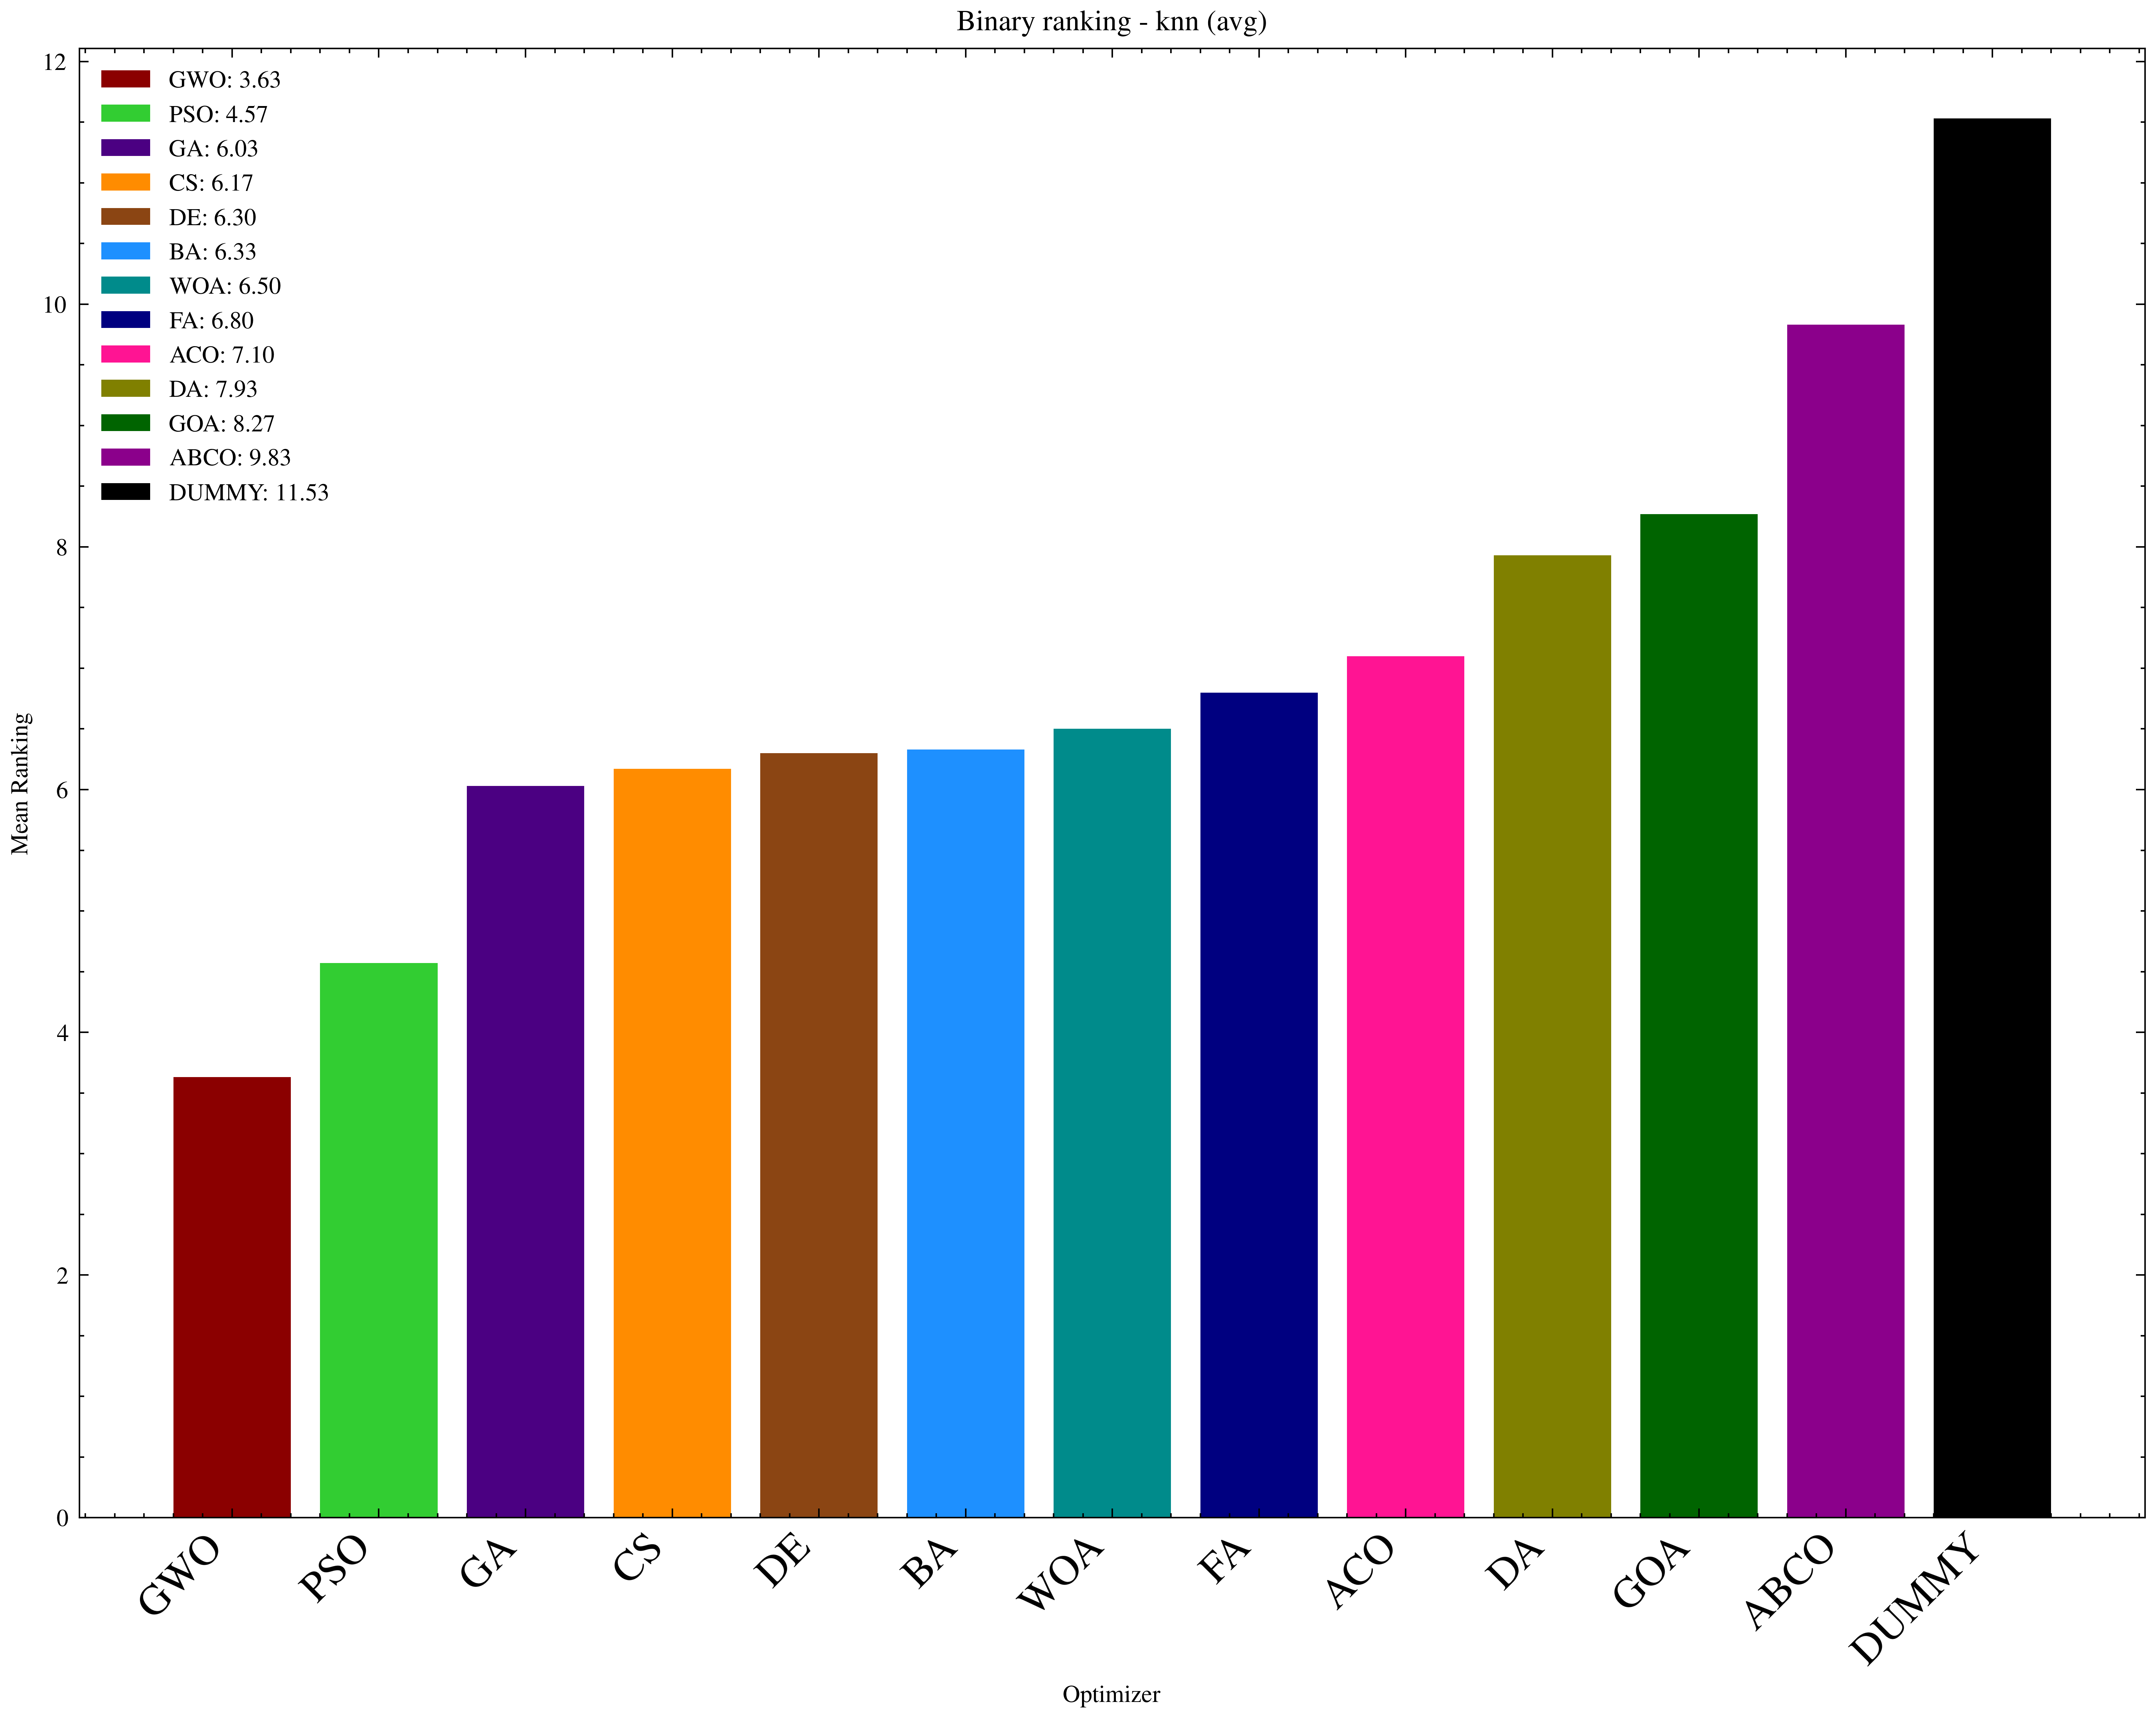
\includegraphics[width=0.8\textwidth]{imagenes/chapter5/rankings_knn_avg_bin.png}
            \end{center}
            \caption{Ranking de los algoritmos en versión binaria para kNN}
        \end{figure}
        \column{0.5\textwidth}
        \begin{figure}
            \begin{center}
                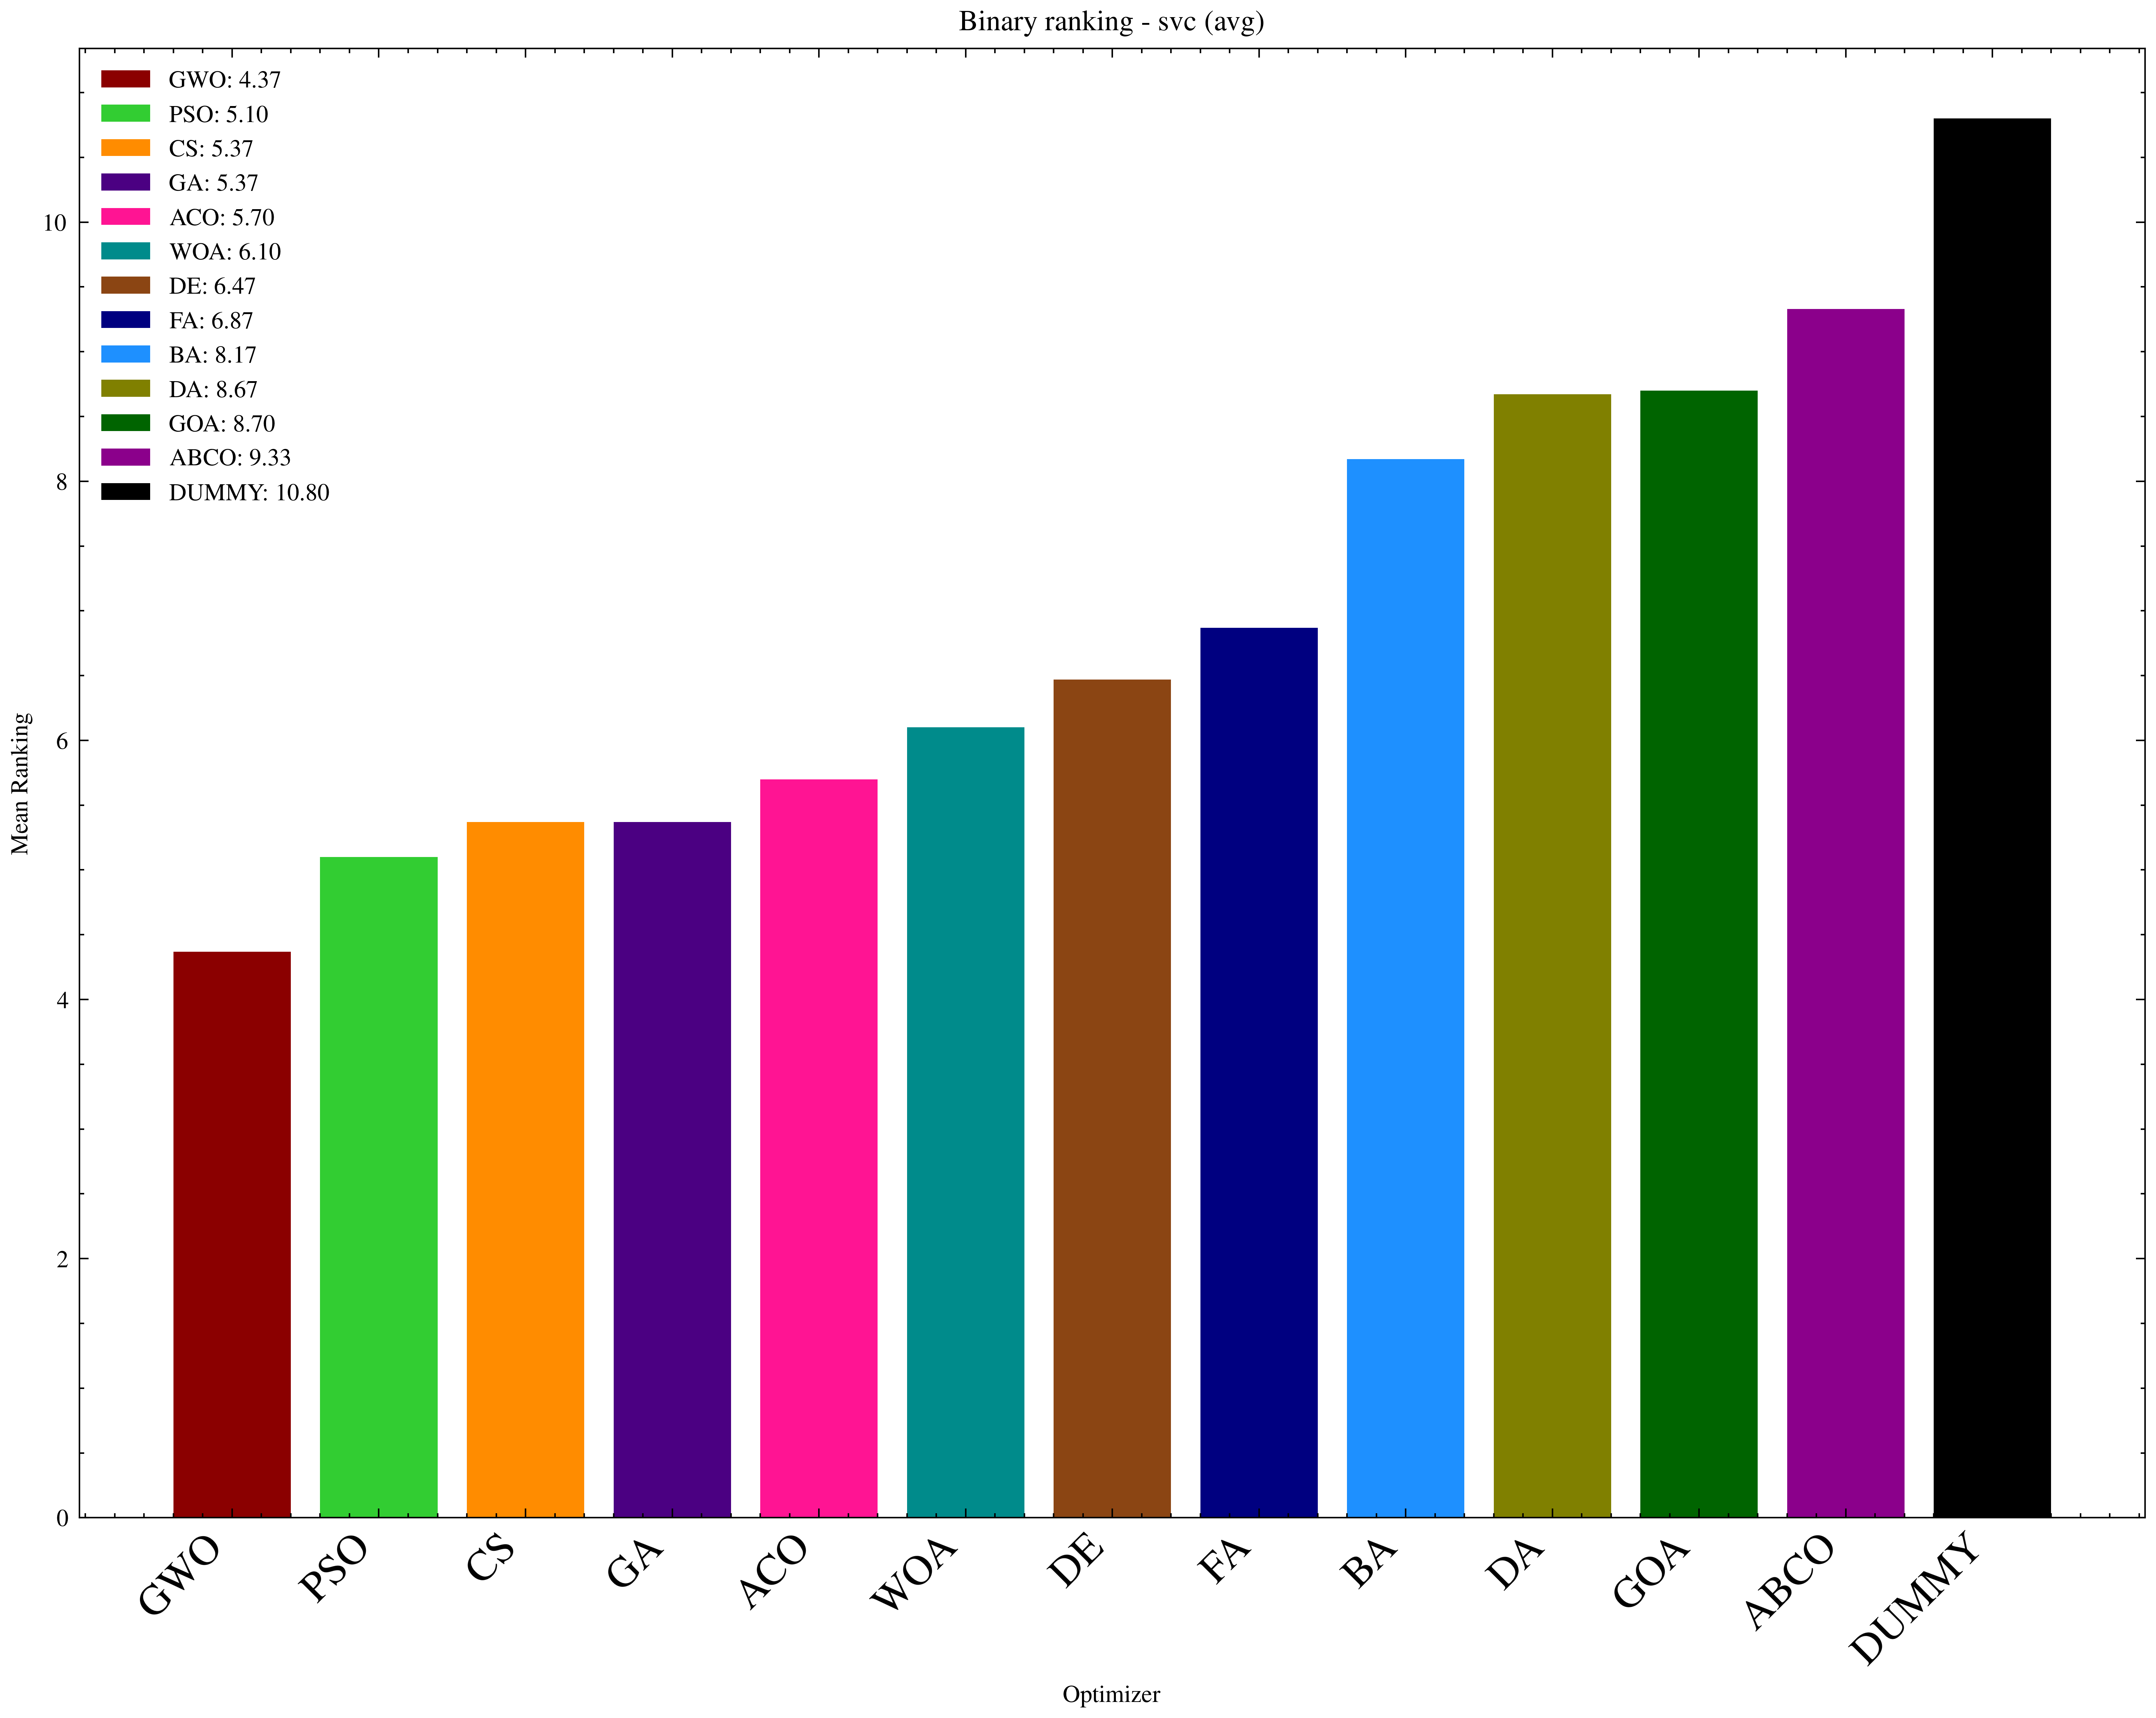
\includegraphics[width=0.8\textwidth]{imagenes/chapter5/rankings_svc_avg_bin.png}
            \end{center}
            \caption{Ranking de los algoritmos en versión binaria para SVC}
        \end{figure}
    \end{columns}
\end{frame}

\begin{frame}
    \frametitle{Resultados en binarios}
    \begin{enumerate}
        \item Los mejores algoritmos en \textit{fitness} son \textbf{bGWO} y \textbf{bPSO}. Los peores algoritmos son \textbf{bGOA} y \textbf{bABCO}.
        \item El mejor reduciendo características es \textbf{ACO}.
        \item El algoritmo más rápido vuelve a ser \textbf{bFA}. Ocurre igual con el más lento, que es \textbf{ABCO}.
    \end{enumerate}
\end{frame}
\section{Conclusiones}
\subsection{Conclusiones}

\begin{frame}
    \frametitle{Conclusiones Principales}
    \begin{itemize}
        \item<1-> \textcolor{green}{Algoritmos específicos vs. originales:} Ambos enfoques son capaces de reducir. Los binarios son mucho más eficaces
        \item<2-> \textcolor{blue}{Recientes vs. clásicos:} Algunos recientes (GWO, CS) muestran excelente rendimiento, pero otros clásicos (PSO, GA) siguen siendo competitivos
        \item<3-> \textcolor{orange}{Prometedores:} GWO y CS destacan en versiones continuas y binarias
        \item<4-> \textcolor{purple}{Eficacia binaria vs. continua:} Generalmente similar, con ligeras ventajas para versiones continuas en algunos casos y viceversa
        \item<5-> \textcolor{red}{Opciones por contexto:}
            \begin{itemize}
                \item Mejor fitness general: CS, GWO (continuo), bGWO, bPSO (binario)
                \item Mejor reducción de características: CS, GWO (continuo), ACO (binario)
                \item Mayor eficiencia temporal: FA (continuo y binario)
            \end{itemize}
    \end{itemize}
\end{frame}

\end{document} 

